% =====================================================================
%  Transcriptomic Profiling of Dwarf Tomato (Solanum lycopersicum
%  cv. 'Red Robin') in Spaceflight — npj Microgravity-style manuscript
%
%  Self-contained: compiles with a standard TeX distribution using
%      pdflatex manuscript_npj.tex   (x2, for references/cross-refs)
%  Figures live in ./figures/ (PNG for raster panels, PDF for vector).
%
%  This preamble emulates the Nature Portfolio / npj two-column, sans-serif
%  house style with only widely-available packages. To submit, the text and
%  figures can be dropped into the official Springer Nature class (sn-jnl.cls,
%  option "pnas"/"npj") with minimal changes.
% =====================================================================
\documentclass[10pt,twocolumn]{article}

\usepackage[a4paper,margin=1.8cm,columnsep=0.7cm]{geometry}
\usepackage[T1]{fontenc}
\usepackage[utf8]{inputenc}
\usepackage{helvet}
\renewcommand{\familydefault}{\sfdefault}   % Arial-like sans-serif (npj house style)
\usepackage{graphicx}
\usepackage{amsmath}
\graphicspath{{figures/}}
\usepackage{subcaption}
\usepackage{caption}
\usepackage{booktabs}
\usepackage{float}
\usepackage{authblk}
\usepackage{titlesec}
\usepackage{xcolor}
\usepackage[super,sort&compress]{natbib}    % superscript numeric citations
\usepackage[colorlinks=true,allcolors=blue!55!black]{hyperref}

% --- npj-style figure labels: "Fig. 1 | ..." ------------------------
\renewcommand{\figurename}{Fig.}
\DeclareCaptionLabelFormat{npjbar}{#1 #2 $\vert$}
\captionsetup{labelformat=npjbar,labelsep=space,font=small,labelfont=bf}
\captionsetup[sub]{labelformat=simple,labelfont=bf,font=footnotesize}
\renewcommand{\thesubfigure}{\alph{subfigure}}

% --- npj-style section headings (bold sans, coloured rule) -----------
\definecolor{npjblue}{RGB}{0,80,140}
\titleformat{\section}{\normalfont\large\bfseries\color{npjblue}}{}{0pt}{}
\titleformat{\subsection}{\normalfont\normalsize\bfseries}{}{0pt}{}
\titlespacing*{\section}{0pt}{1.4ex}{0.6ex}
\titlespacing*{\subsection}{0pt}{1.0ex}{0.4ex}

\setlength{\parindent}{1.2em}
\setlength{\parskip}{0pt}
\renewcommand{\baselinestretch}{1.05}

% =====================================================================
\title{\bfseries\LARGE Transcriptomic profiling of dwarf tomato
(\textit{Solanum lycopersicum} cv.\ `Red Robin') in spaceflight:
evaluating the main effects of microgravity under red- and blue-light covariates}

\author[1]{Richard J.\ Barker}
\affil[1]{\normalfont\small Affiliation to be completed. Correspondence: \texttt{dr.richard.barker@gmail.com}}
\date{}

% =====================================================================
\begin{document}
\twocolumn[
\begin{@twocolumnfalse}
\maketitle
\vspace{-2.5em}
\begin{abstract}
\noindent\small
\textbf{Cultivating nutrient-dense crops in microgravity is a prerequisite for
long-duration human space exploration, yet the molecular adaptations of fruiting
crops to spaceflight remain incompletely resolved.} Using RNA-sequencing data
from the NASA VEG-05 experiment (Open Science Data Repository OSD-767 / GLDS-709),
we profiled leaf ($n=21$) and adventitious-root ($n=15$) tissues of dwarf tomato
grown aboard the International Space Station under red- and blue-rich light versus
ground controls. Modelling light spectrum as a covariate (\texttt{$\sim$ light +
condition}) to isolate the main effect of spaceflight, we identified 2,132
differentially expressed genes (DEGs) in leaf (1,032 up / 1,100 down) and 2,582 in
adventitious root (1,706 up / 876 down), with roots showing a larger and more
strongly up-regulated response. Functional enrichment converged on oxidative-stress
management and specialised metabolism: root up-regulated genes were dominated by
``response to oxidative stress'' (GO, FDR $\approx 6.5\times10^{-13}$), hydrogen-peroxide
catabolism and ethylene signalling, and by KEGG phenylpropanoid (FDR $\approx
4\times10^{-30}$), flavonoid and stilbenoid biosynthesis with glutathione metabolism.
The plant circadian-rhythm pathway was down-regulated in both organs. Cross-referencing
root DEGs against a published tomato root cell-type atlas localised the response to
cortex, exodermis, endodermis, meristematic-cortex and vascular cell populations.
These light-averaged responses, which independently corroborate the original VEG-05
report, identify antioxidant and phenylpropanoid metabolism as core targets for
engineering spaceflight-resilient crops.
\end{abstract}
\vspace{1.2em}
\end{@twocolumnfalse}
]

% =====================================================================
\section{Introduction}
Long-duration space missions require bioregenerative life-support systems that
supply fresh, nutrient-dense food. The dwarf tomato (\textit{Solanum lycopersicum}
cv.\ `Red Robin') is a leading candidate for space agriculture owing to its compact
habit, continuous fruiting and nutritional value. Understanding how this crop adapts
to the coupled stressors of spaceflight---microgravity, altered fluid behaviour and
the closed cultivation environment---is essential to optimise off-Earth cultivation.

Plant physiology is strongly shaped by light quality. In the Vegetable Production
System (Veggie) aboard the International Space Station (ISS), red and blue wavelengths
govern photosynthetic efficiency, phototropism and stress signalling through
phytochrome, cryptochrome and phototropin photoreceptors. It remains unclear how the
foundational transcriptomic response to microgravity operates across, or interacts
with, these light cues. The VEG-05 experiment (OSD-767) was designed to evaluate the
impact of red- versus blue-rich light on tomato growth, nutrition and microbial
safety in space. Here we leverage its transcriptomic data to isolate the fundamental
genetic adaptations of \textit{S.\ lycopersicum} to spaceflight. Rather than testing a
flight-by-light interaction, we model light condition as a covariate, determining the
robust primary effects of spaceflight on leaf and adventitious-root transcriptomes
averaged across light spectra, and thereby define the core molecular footprint of
spaceflight adaptation in a vital crop species.

% =====================================================================
\section{Results}

\subsection{Data quality, dispersion and sample ordination}
After trimming and alignment, per-gene dispersion estimates conformed to the expected
mean--variance relationship in both tissues, supporting the negative-binomial models.
Unsupervised ordination of variance-stabilised counts separated samples primarily by
spaceflight condition: the leading principal components distinguished Flight from
Ground samples, while red- and blue-light replicates interleaved within each
condition (Fig.~\ref{fig:qc}), consistent with treating light spectrum as a covariate.
The larger within-group spread among root samples reflects the limited and imbalanced
root ground-control replication ($n=3$ per light condition).

\subsection{Spaceflight extensively remodels the leaf transcriptome}
At an adjusted $p<0.05$ and $|\log_2\text{FC}|\ge 1$, the leaf Flight-versus-Ground
contrast identified \textbf{2,132 significant DEGs} (1,032 up, 1,100 down in
spaceflight; Table~\ref{tab:deg}). The response was both broad and highly significant:
1,337 genes passed FDR $<0.001$. Individual effect sizes were moderate, the most
strongly induced leaf genes reaching $\log_2\text{FC}\approx +5.6$ (e.g.\
\textit{Solyc07g052370}, $\log_2\text{FC}\approx +5.0$, FDR $\approx 1\times10^{-17}$)
and the most repressed $\approx -4.5$. Volcano and MA representations
(Fig.~\ref{fig:leaf}) show a broadly symmetric distribution of induced and repressed
genes across the expression range.

\subsection{Adventitious roots display a larger, up-regulation-biased response}
The adventitious-root contrast identified \textbf{2,582 significant DEGs}, exceeding
the leaf response in magnitude and asymmetry: 1,706 genes up- versus 876
down-regulated ($\approx$2:1 induction bias; 638 at FDR $<0.001$). Effect sizes were
markedly larger than in leaf---numerous root genes were induced from near-absent
baseline expression, the strongest exceeding 10 $\log_2$-units (the single most
extreme $\approx +25$ from a near-zero ground baseline), indicating switch-like
activation of otherwise silent loci in spaceflight. Sample-distance clustering,
ordination, volcano and MA plots (Figs.~\ref{fig:qc},~\ref{fig:root}) consistently
separated Flight from Ground root samples and highlighted the up-regulation bias.

\subsection{Enrichment implicates oxidative-stress management and specialised metabolism}
Gene Ontology (GO) and KEGG over-representation analysis of the directional DEG sets
revealed a coherent, stress-centred programme. In \textbf{roots}, up-regulated genes
were overwhelmingly enriched for oxidative-stress management: the GO biological
processes ``response to oxidative stress'' (32 genes, FDR $\approx 6.5\times10^{-13}$)
and ``hydrogen peroxide catabolic process'' (28 genes) were the leading terms,
alongside ``ethylene-activated signaling pathway'' (FDR $\approx 1\times10^{-6}$) and,
at the molecular-function level, an exceptionally strong heme-binding signature (67
genes, FDR $\approx 9\times10^{-18}$) reflecting peroxidase and cytochrome activity
(Fig.~\ref{fig:enr_root}a). The corresponding KEGG analysis was dominated by
\textbf{phenylpropanoid biosynthesis} (45 genes, FDR $\approx 4\times10^{-30}$),
followed by stilbenoid, flavonoid and aromatic-amino-acid biosynthesis and by
\textbf{glutathione metabolism} (Fig.~\ref{fig:enr_root}b)---a concerted mobilisation
of antioxidant and secondary-metabolite pathways.

In \textbf{leaves}, up-regulated genes showed a related but attenuated signature:
enrichment for heme binding, monooxygenase/oxidoreductase and iron-ion binding
(Fig.~\ref{fig:enr_leaf}a), induction of abscisic-acid--binding genes, and KEGG
enrichment for phenylpropanoid and flavonoid biosynthesis, amino-acid biosynthesis,
MAPK signalling and plant-hormone signal transduction (Fig.~\ref{fig:enr_leaf}b).
Down-regulated genes pointed to suppression of normal growth and timekeeping: the
\textbf{plant circadian-rhythm} KEGG pathway was significantly down-regulated in
\emph{both} organs, roots additionally down-regulating Calvin-cycle carbon fixation
and starch/sucrose metabolism, and leaves down-regulating transmembrane transport,
galactose and folate metabolism and glycolysis
(Figs.~\ref{fig:enr_root}c,~\ref{fig:enr_leaf}c).

\subsection{Root DEGs localise to ground-tissue and vascular cell types}
To interpret the bulk response cellularly, root DEGs were cross-referenced against
published tomato root cell-type marker sets\cite{kajala2021} by Fisher's exact test.
Twenty-five cell-type $\times$ DEG associations were significant
(Fig.~\ref{fig:celltype}). Down-regulated root genes were most strongly enriched in
\textbf{cortex} (odds ratio $\approx 3.6$, FDR $\approx 7\times10^{-29}$),
\textbf{endodermis}, \textbf{meristematic cortex} and \textbf{xylem/vascular} markers,
whereas up-regulated genes were most enriched in \textbf{exodermis} (OR $\approx 2.8$)
and an actin-defined cortex population (Cortex\_ACT2, OR $\approx 4.4$). The response
therefore concentrates in the ground-tissue layers and the vasculature---precisely the
cell populations re-specified during adventitious-root formation. Cross-referencing
against a leaf cluster atlas gave a weaker, less tissue-specific pattern.

% =====================================================================
\section{Discussion}
This study isolates the core, light-averaged transcriptomic response of dwarf tomato
to spaceflight in the two organs most relevant to crop performance---photosynthetic
leaves and the adventitious roots that proliferate in microgravity. By modelling light
spectrum as a covariate we traded sensitivity to light-specific effects for power on
the main effect of spaceflight, recovering a pervasive response of $\sim$2,100 leaf
and $\sim$2,600 root DEGs.

\textbf{Adventitious roots are the focal organ.} Roots contained more DEGs than
leaves, showed a pronounced up-regulation bias and far larger effect sizes, including
switch-like activation of loci essentially silent in ground controls. This intensity
mirrors the documented phenotype of extensive adventitious rooting in spaceflight, and
our cell-type cross-reference ties the signal specifically to cortex, exodermis,
endodermis and vascular populations---the tissues that physically remodel during
rooting. Spaceflight adaptation in tomato roots is thus, in large part, a programme of
ground-tissue and vascular re-organisation rather than a uniform whole-organ response.

\textbf{A shared oxidative-stress and phenylpropanoid signature.} The most robust
theme across both organs is management of reactive oxygen species. Extreme enrichment
of oxidative-stress response, hydrogen-peroxide catabolism and heme/peroxidase activity
in roots, with induction of glutathione metabolism, indicates that antioxidant defence
is a central axis of adaptation. This couples to strong mobilisation of the
phenylpropanoid and flavonoid pathways---versatile sources of antioxidant and
lignin-precursor metabolites---the strongest KEGG signal in roots and also significant
in leaves. Because phenylpropanoid-derived compounds feed both ROS scavenging and
cell-wall reinforcement, their induction plausibly serves the dual demands of
oxidative defence and the mechanical remodelling accompanying adventitious rooting.

\textbf{Hormonal and circadian reprogramming.} Ethylene signalling in roots and
abscisic-acid--binding genes in leaves implicate classical stress hormones, reinforced
by leaf MAPK and hormone signal-transduction enrichment. Down-regulation of the
circadian-rhythm pathway in \emph{both} organs is notable: circadian disruption
recurs across spaceflight biology, and its appearance in a light-controlled analysis
argues it is a genuine microgravity-associated effect rather than a light artefact.
Concurrent suppression of primary carbon and energy metabolism is consistent with
resource re-allocation from growth toward defensive and structural metabolism.

\textbf{Concordance with the original VEG-05 report.} These findings independently
corroborate the published analysis of this dataset\cite{dixit2026}, which likewise
reported pronounced adventitious-root change and highlighted oxidative-stress
response, secondary-metabolite biosynthesis and hormonal regulation. We reach these
conclusions through a different statistical route---an additive covariate model
estimating the pooled main effect of spaceflight, rather than within-light contrasts
intersected across treatments---and consequently report larger DEG counts under a more
permissive fold-change threshold. The analyses are complementary: the published
within-light design isolates a conservative core of light-invariant genes, whereas the
present design maximises power to describe the full breadth of the response and to
localise it to specific cell types.

\textbf{Limitations.} The root ground-control group comprises only three replicates
per light condition, limiting power and inflating dispersion for root contrasts;
formal light$\times$spaceflight interaction testing in root is under-powered (an
exploratory interaction analysis is provided in the associated data repository).
\textit{Solanum}-to-Entrez identifier mapping recovered 60--75\% of genes, so
enrichment under-samples unmapped loci. The cell-type cross-reference relies on
published markers rather than a spaceflight-specific single-cell atlas, so cell-type
assignments are inherited from ground-grown reference tissue.

\textbf{Conclusions.} Averaged across red- and blue-rich light, spaceflight imposes a
coordinated, stress-oriented transcriptional programme on dwarf tomato that is
strongest in adventitious roots and built around antioxidant defence,
phenylpropanoid/flavonoid metabolism, stress-hormone signalling and circadian
dysregulation, with the root response localised to ground-tissue and vascular layers.
These pathways constitute a concise set of candidate targets---peroxidase/glutathione
antioxidant systems and phenylpropanoid flux in particular---for breeding or
engineering tomato cultivars better suited to bioregenerative life-support systems.

% =====================================================================
\section{Methods}
\subsection{Data acquisition and experimental design}
Raw paired-end RNA-seq reads (151\,bp, NovaSeq X Plus) for VEG-05 were obtained from
the NASA Open Science Data Repository (OSD-767; GeneLab GLDS-709). The design comprised
21 leaf samples (Flight/Red $n{=}5$, Flight/Blue $n{=}4$, Ground/Red $n{=}6$,
Ground/Blue $n{=}6$) and 15 adventitious-root samples (Flight/Red $n{=}5$, Flight/Blue
$n{=}4$, Ground/Red $n{=}3$, Ground/Blue $n{=}3$).

\subsection{Pre-processing and quality control}
Processing followed the NASA GeneLab RNAseq Consensus Pipeline (GL-DPPD-7101-G /
NF\_RCP 2.0.1). Read quality was assessed with FastQC v0.12.1 and aggregated with
MultiQC v1.26; adapters and low-quality bases were removed with Trim~Galore! v0.6.10
(Cutadapt v4.2; \texttt{--phred33}, paired-end), followed by a second FastQC pass.

\subsection{Alignment and quantification}
The Ensembl Plants \textit{S.\ lycopersicum} SL3.0 assembly with ITAG gene models was
used as reference. Trimmed reads were aligned with STAR\cite{star} v2.7.11b in two-pass mode
(\texttt{--sjdbOverhang 150}, \texttt{--outFilterMultimapNmax 20},
\texttt{--outFilterMismatchNoverReadLmax 0.04}); transcriptome alignments were
quantified with RSEM\cite{rsem} v1.3.1 (\texttt{--estimate-rspd}). Strandedness and library
geometry were verified with RSeQC v5.0.4.

\subsection{Differential expression}
Gene-level counts were imported with tximport v1.38.2 into DESeq2\cite{deseq2} v1.50.2 (R v4.4.2).
Leaf and root tissues were analysed independently. To isolate the primary effect of
spaceflight while controlling for light, the design was \texttt{$\sim$ light +
condition}, with the Flight-versus-Ground contrast as primary. Low-count genes were
pre-filtered; log$_2$ fold changes were shrunk for visualisation. DEGs were defined by
Benjamini--Hochberg FDR $<0.05$ and $|\log_2\text{FC}|\ge 1$. Volcano, MA and PCA plots
were produced with EnhancedVolcano v1.28.2 and DESeq2.

\subsection{Functional enrichment}
GO (BP/MF/CC) and KEGG (\texttt{organism = "sly"}) over-representation was performed
with clusterProfiler\cite{clusterprofiler}; Solyc identifiers were mapped to Entrez via
biomaRt (Ensembl Plants). Enrichment used relaxed cut-offs for small gene sets; the
combined results are provided as a supplementary table.

\subsection{Cell-type cross-reference}
Directional DEG sets were intersected with published tomato root cell-type marker
lists\cite{kajala2021}; per-cell-type over-representation was tested by Fisher's exact
test with Bonferroni correction and summarised as $-\log_{10}$ adjusted $p$.

% =====================================================================
\section*{Data availability}
Primary data are available from the NASA Open Science Data Repository under accession
\href{https://osdr.nasa.gov/bio/repo/data/studies/OSD-767}{OSD-767} (GLDS-709). All
processed results, figures, code trace and this manuscript are archived in the project
repository and will be deposited on Zenodo (DOI to be assigned).

\section*{Acknowledgements}
We thank the NASA GeneLab/OSDR team and the VEG-05 investigators for generating and
openly sharing the primary dataset.

\section*{Competing interests}
The author declares no competing interests.

% =====================================================================
\begin{thebibliography}{9}
\bibitem{dixit2026} Dixit, A.\,R. \textit{et al.} Stress and light spectral quality
influence the transcriptome of a tomato crop on the International Space Station.
\textit{BMC Plant Biol.} \textbf{26}, 764 (2026).
\bibitem{clusterprofiler} Wu, T. \textit{et al.} clusterProfiler 4.0: A universal
enrichment tool for interpreting omics data. \textit{The Innovation} \textbf{2},
100141 (2021).
\bibitem{kajala2021} Kajala, K. \textit{et al.} Innovation, conservation and
repurposing of gene function in root cell type development. \textit{Cell} \textbf{184},
3333--3348 (2021).
\bibitem{deseq2} Love, M.\,I., Huber, W. \& Anders, S. Moderated estimation of fold
change and dispersion for RNA-seq data with DESeq2. \textit{Genome Biol.} \textbf{15},
550 (2014).
\bibitem{star} Dobin, A. \textit{et al.} STAR: ultrafast universal RNA-seq aligner.
\textit{Bioinformatics} \textbf{29}, 15--21 (2013).
\bibitem{rsem} Li, B. \& Dewey, C.\,N. RSEM: accurate transcript quantification from
RNA-Seq data with or without a reference genome. \textit{BMC Bioinformatics}
\textbf{12}, 323 (2011).
\end{thebibliography}

% =====================================================================
%  FIGURES
% =====================================================================
\begin{figure*}[t]
\centering
\begin{subfigure}{0.32\textwidth}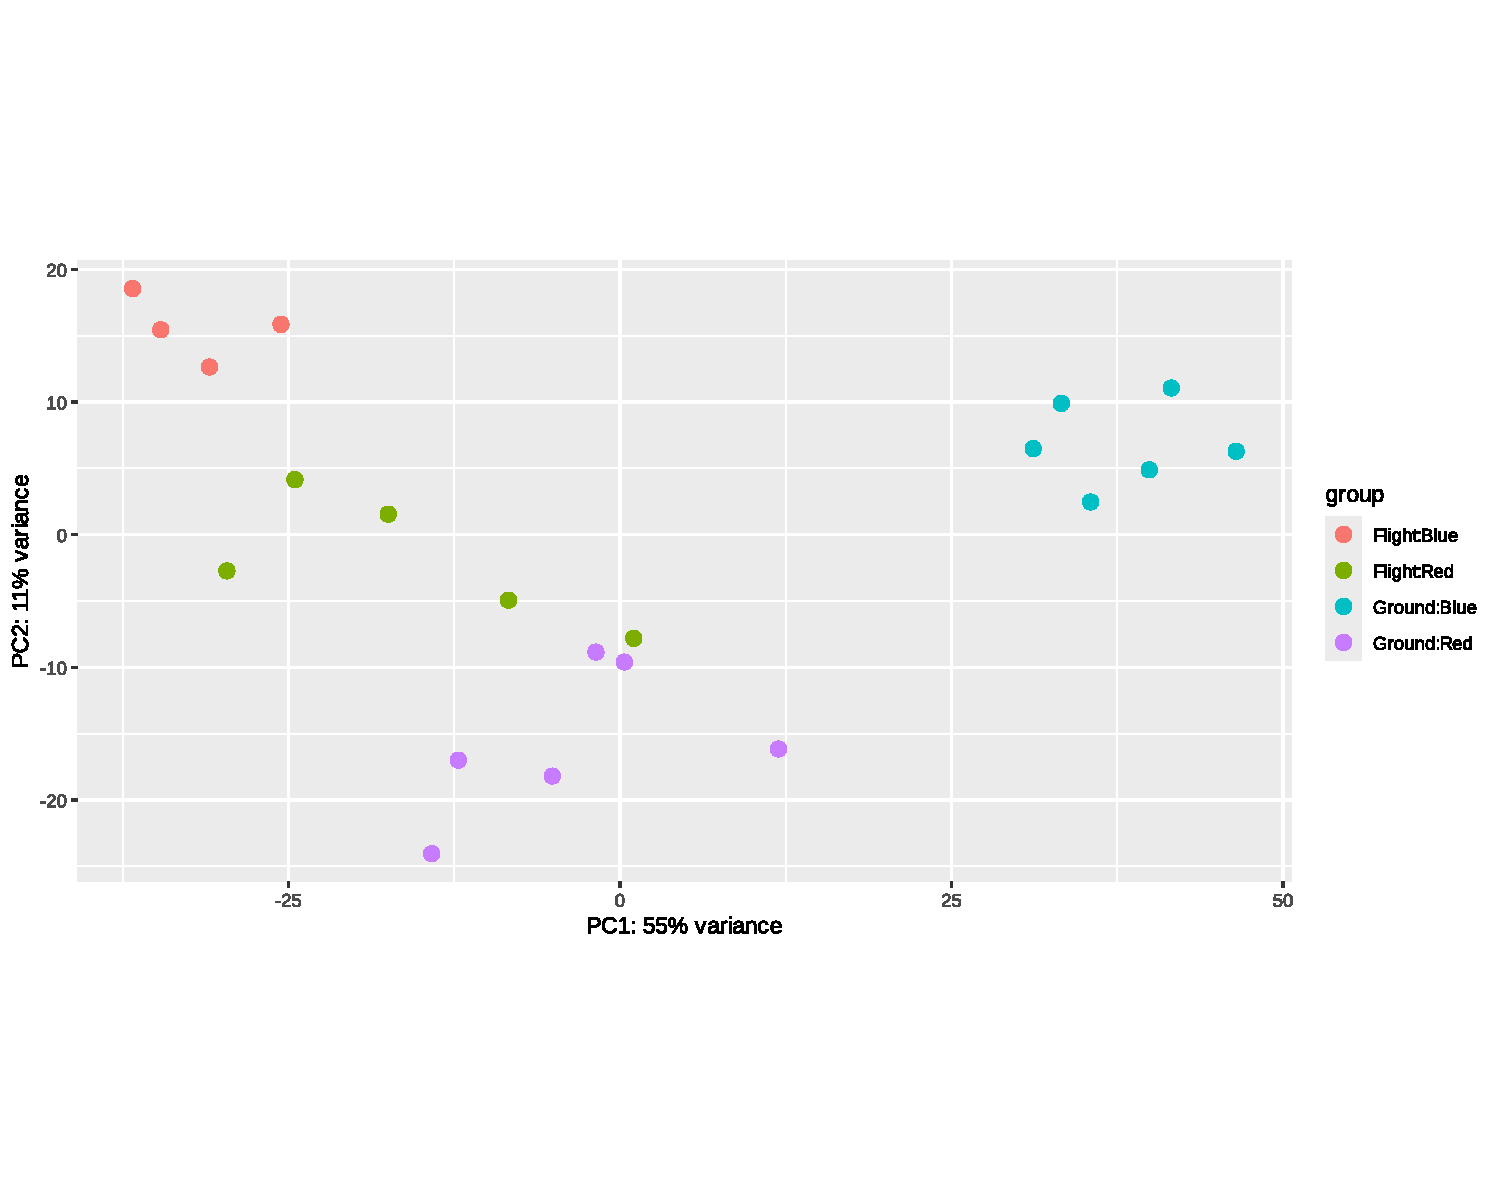
\includegraphics[width=\linewidth]{fig1a_leaf_pca.pdf}\caption{}\end{subfigure}\hfill
\begin{subfigure}{0.32\textwidth}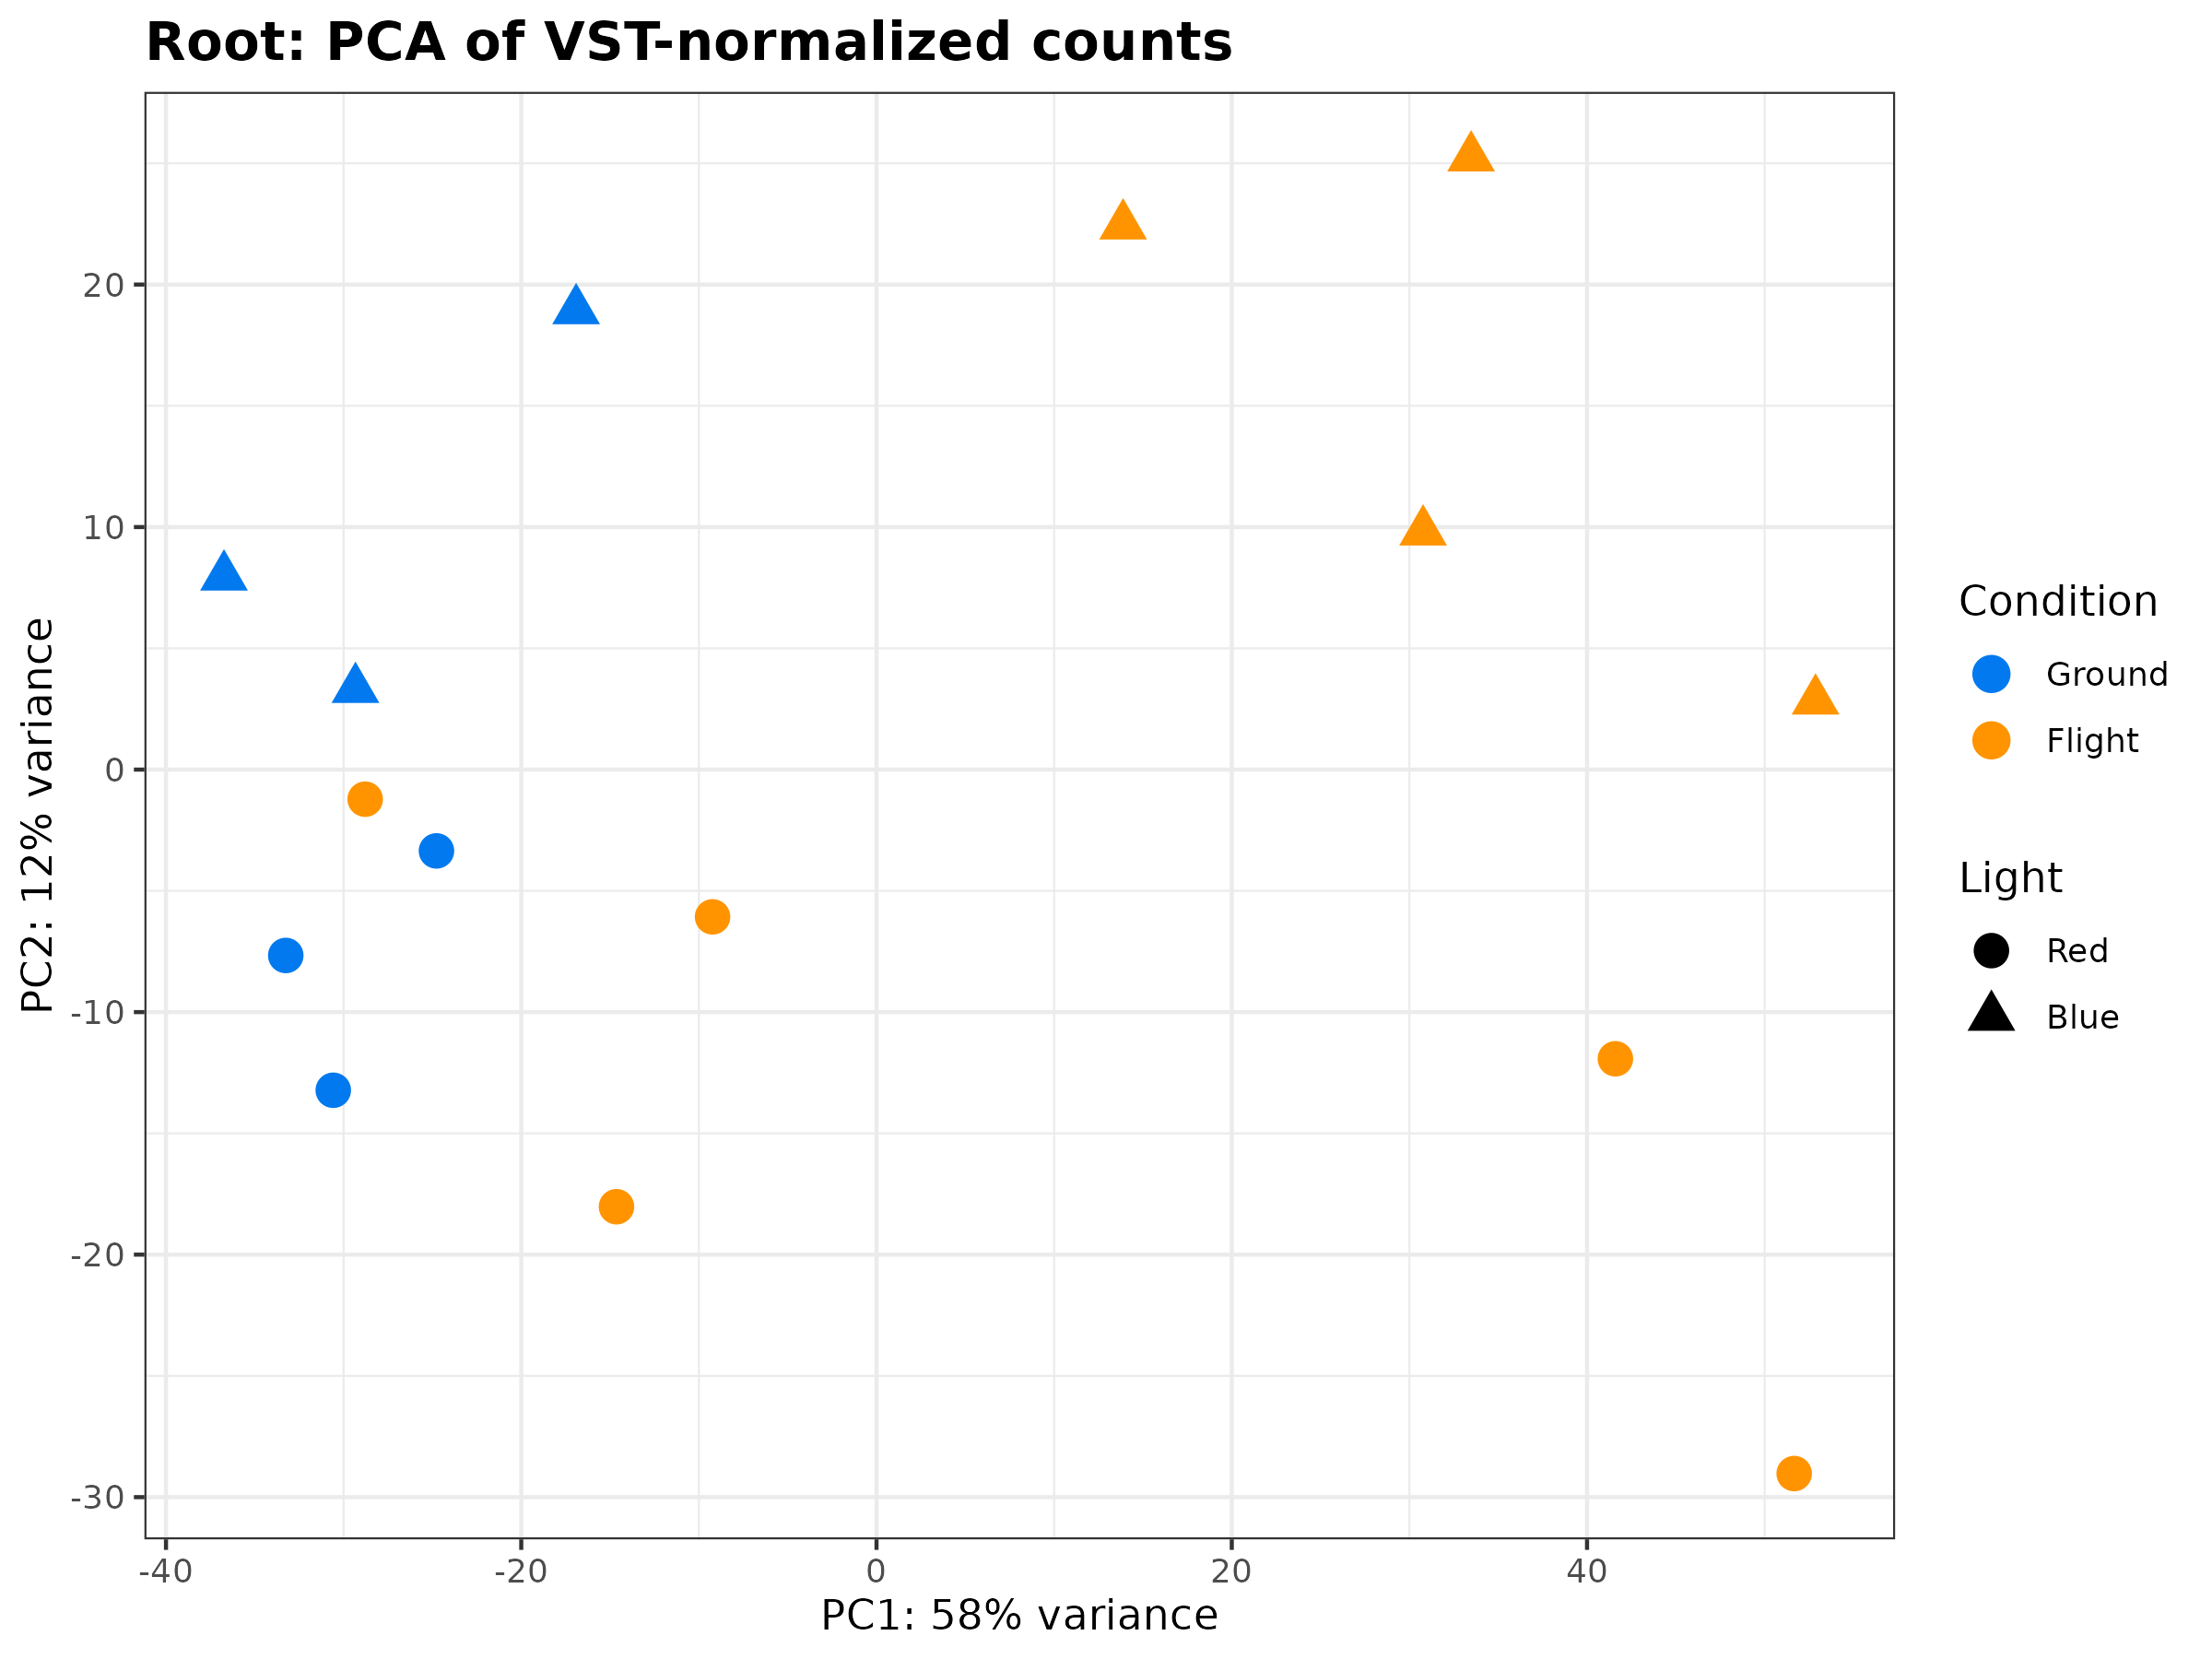
\includegraphics[width=\linewidth]{fig1c_root_pca.png}\caption{}\end{subfigure}\hfill
\begin{subfigure}{0.32\textwidth}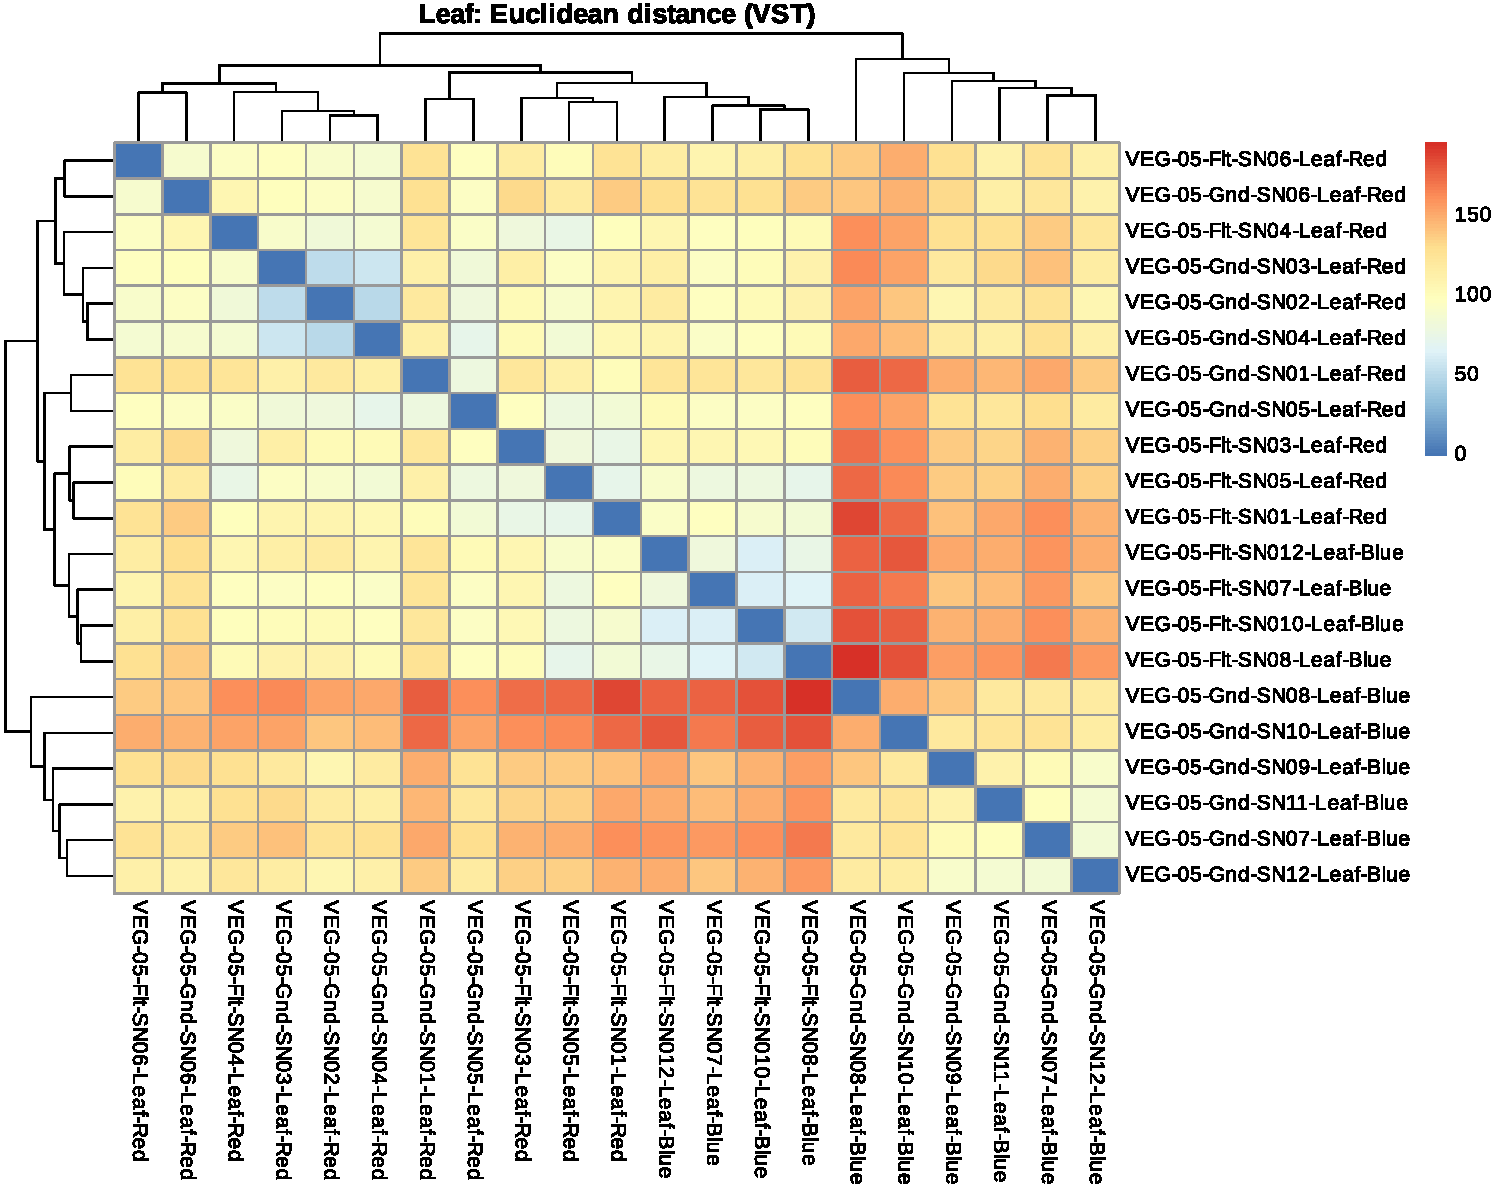
\includegraphics[width=\linewidth]{fig1b_leaf_distheat.pdf}\caption{}\end{subfigure}
\\[0.4em]
\begin{subfigure}{0.32\textwidth}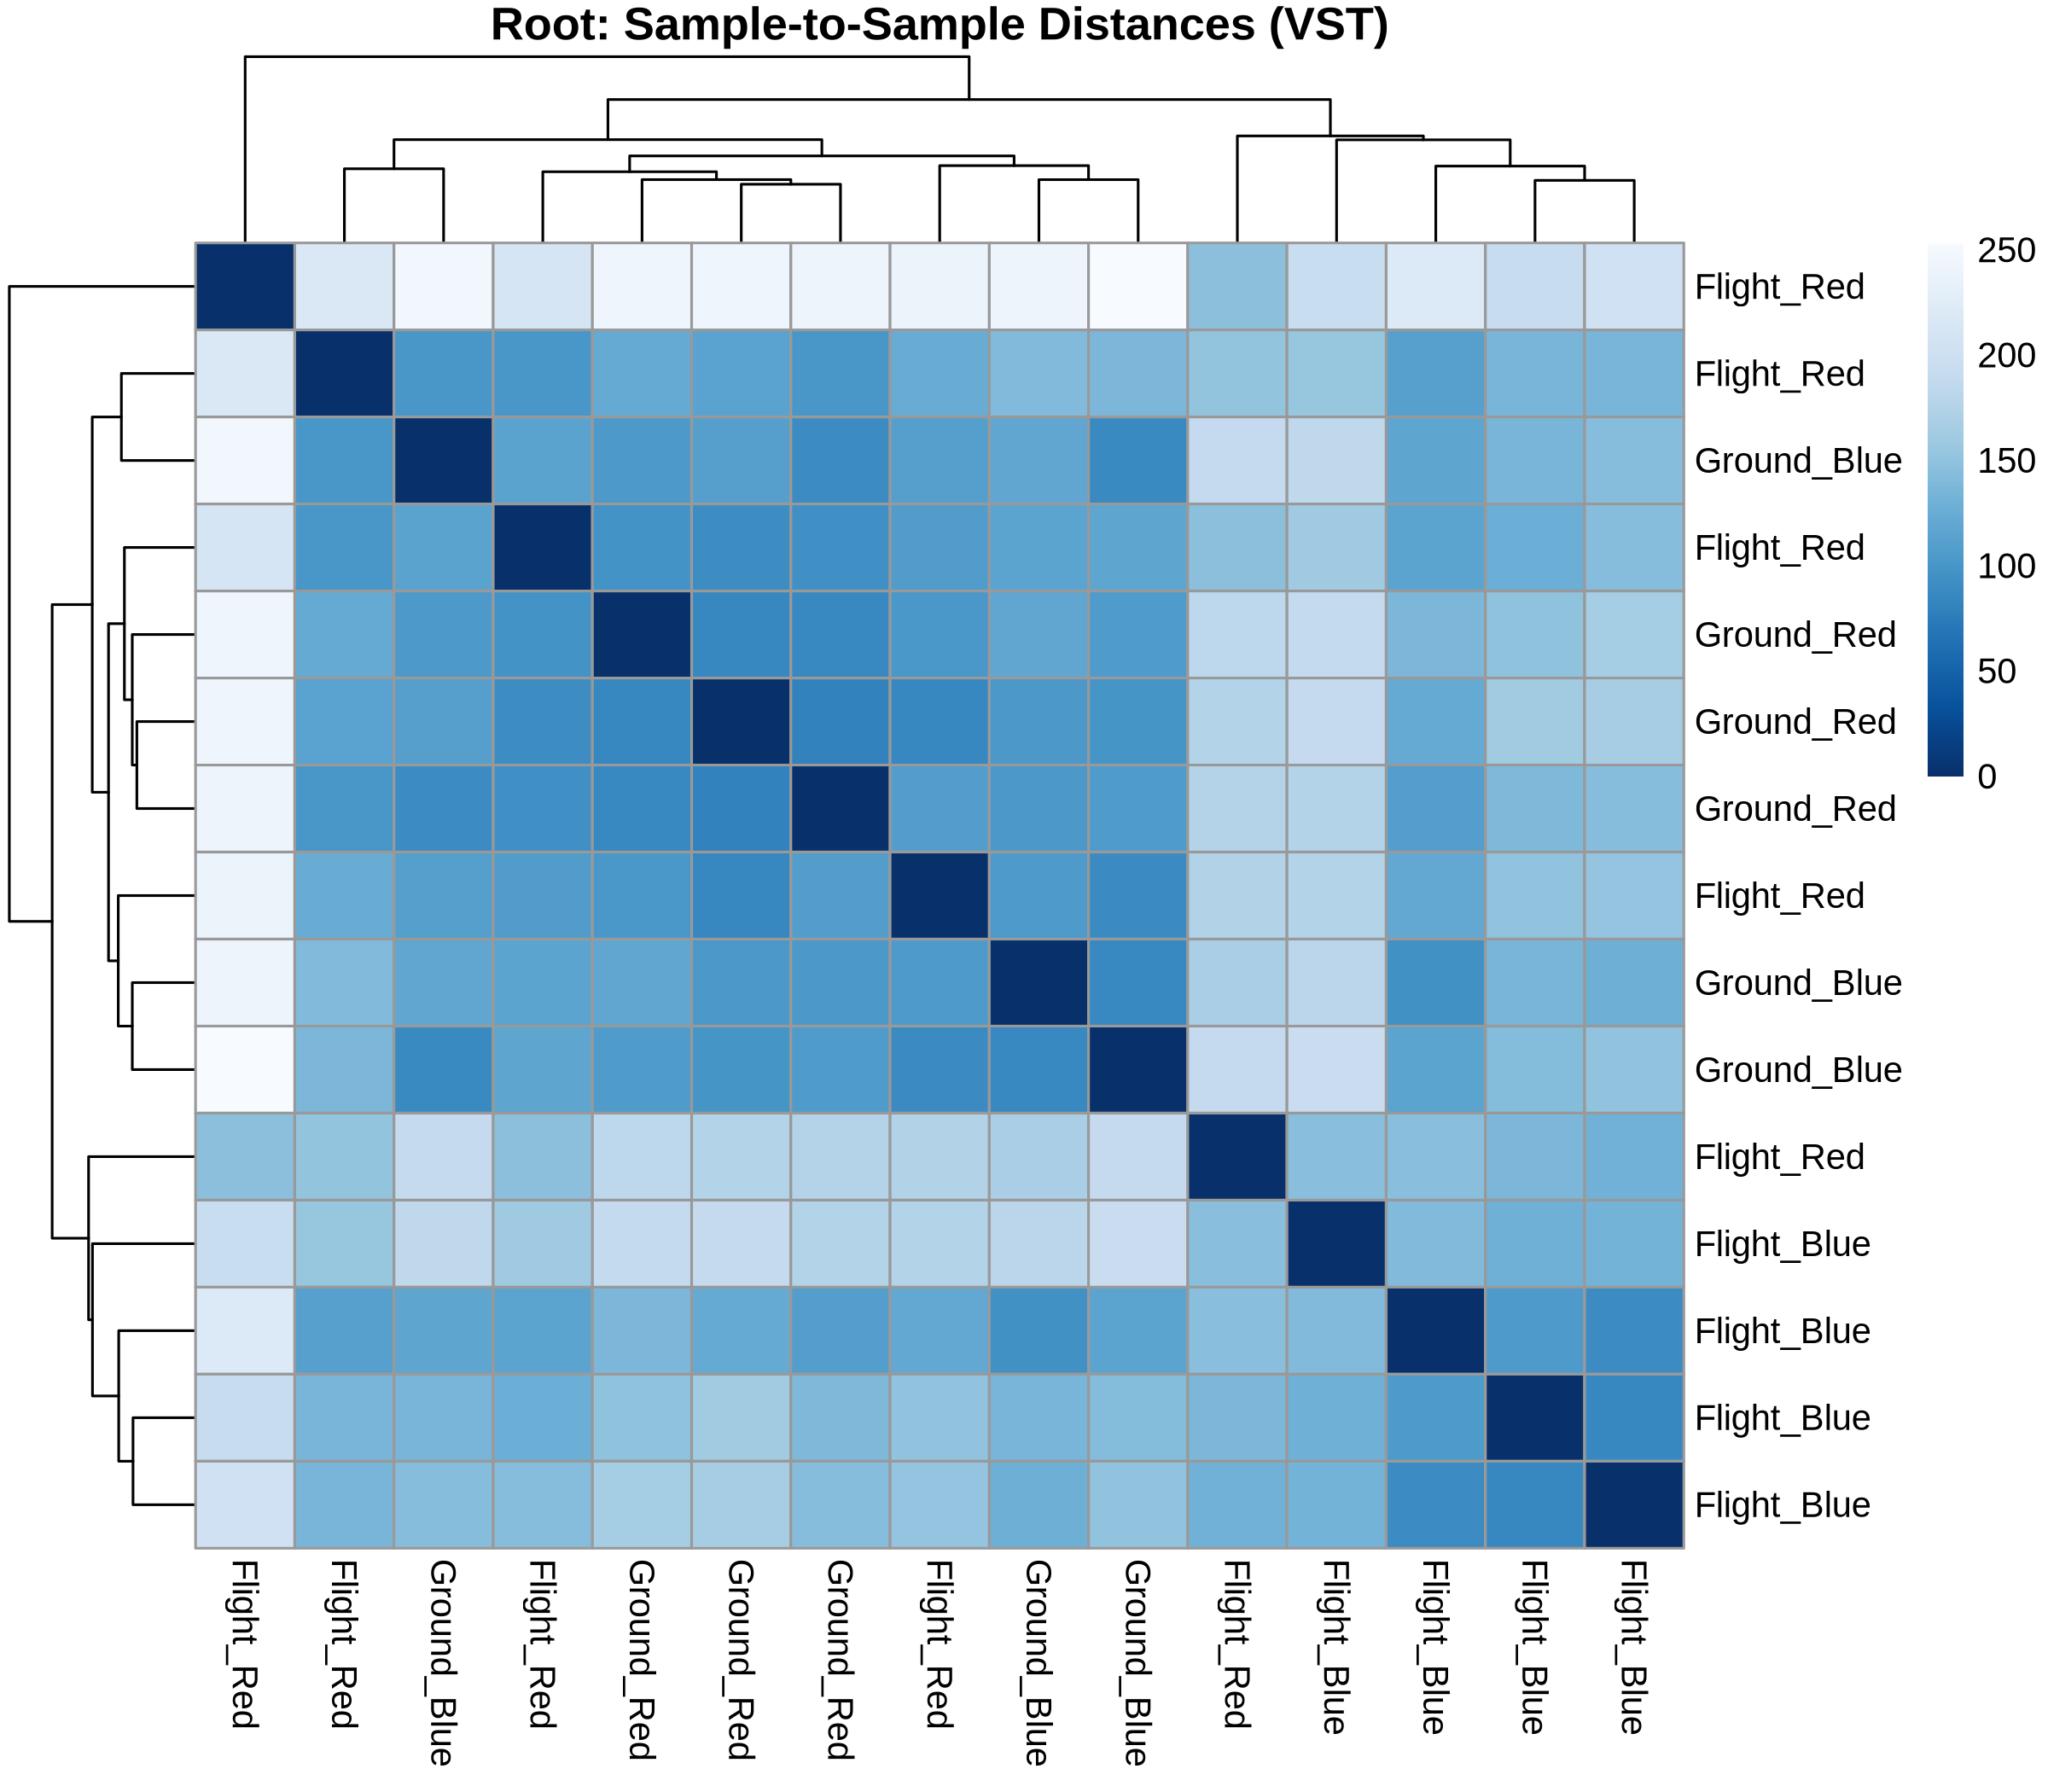
\includegraphics[width=\linewidth]{fig1d_root_distheat.png}\caption{}\end{subfigure}
\caption{\textbf{Sample quality and ordination separate spaceflight from ground
controls.} Principal-component analysis of variance-stabilised counts for
(\textbf{a})~leaf and (\textbf{b})~adventitious-root samples, and sample-to-sample
Euclidean-distance heatmaps for (\textbf{c})~leaf and (\textbf{d})~root. In both organs
the dominant axis of variation separates Flight from Ground, while red- and blue-light
replicates interleave within each condition, supporting the covariate design. Root
samples show greater spread, consistent with the limited root ground-control
replication ($n=3$ per light condition).}
\label{fig:qc}
\end{figure*}

\begin{figure*}[t]
\centering
\begin{subfigure}{0.46\textwidth}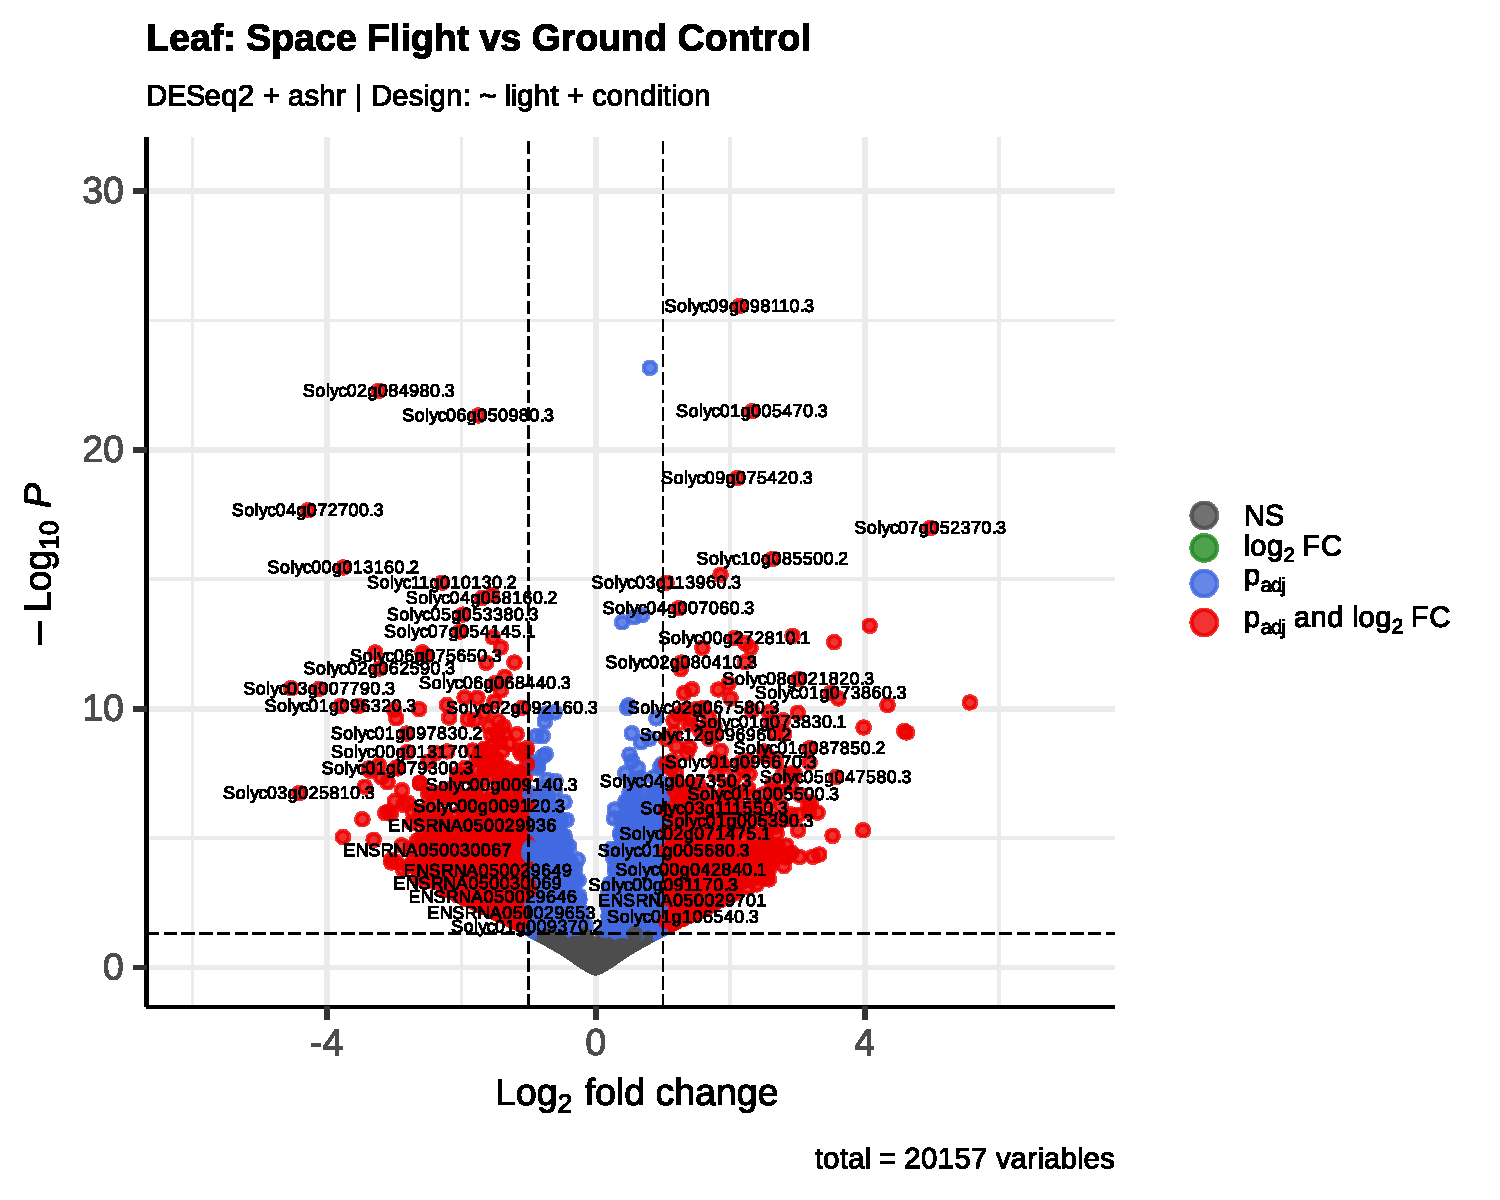
\includegraphics[width=\linewidth]{fig2a_leaf_volcano.pdf}\caption{}\end{subfigure}\hfill
\begin{subfigure}{0.46\textwidth}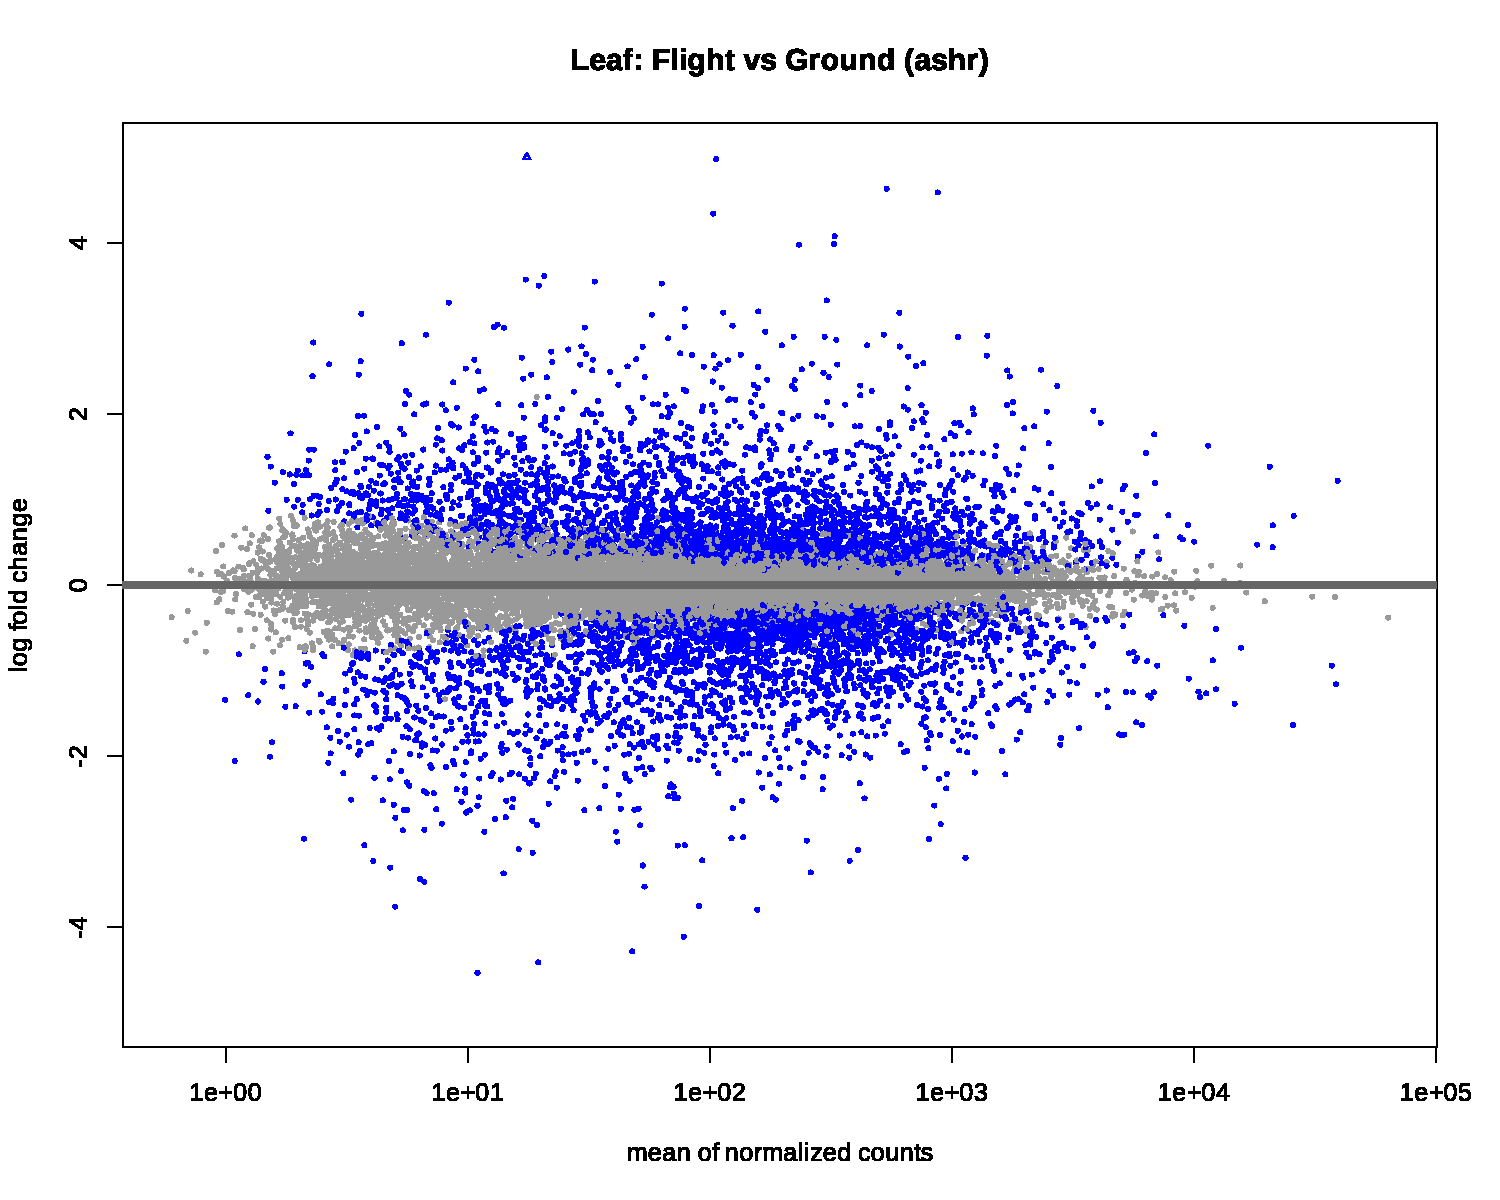
\includegraphics[width=\linewidth]{fig2b_leaf_ma.pdf}\caption{}\end{subfigure}
\caption{\textbf{Spaceflight extensively remodels the leaf transcriptome.}
(\textbf{a})~Volcano plot and (\textbf{b})~MA plot of the leaf Flight-versus-Ground
contrast (DESeq2, \texttt{$\sim$ light + condition}). Of 2,132 significant DEGs
(FDR $<0.05$, $|\log_2\text{FC}|\ge 1$), 1,032 are up- and 1,100 down-regulated in
spaceflight; effect sizes are moderate (maximum $|\log_2\text{FC}|\approx 5.6$) and the
induced/repressed distribution is broadly symmetric across the expression range.}
\label{fig:leaf}
\end{figure*}

\begin{figure*}[t]
\centering
\begin{subfigure}{0.46\textwidth}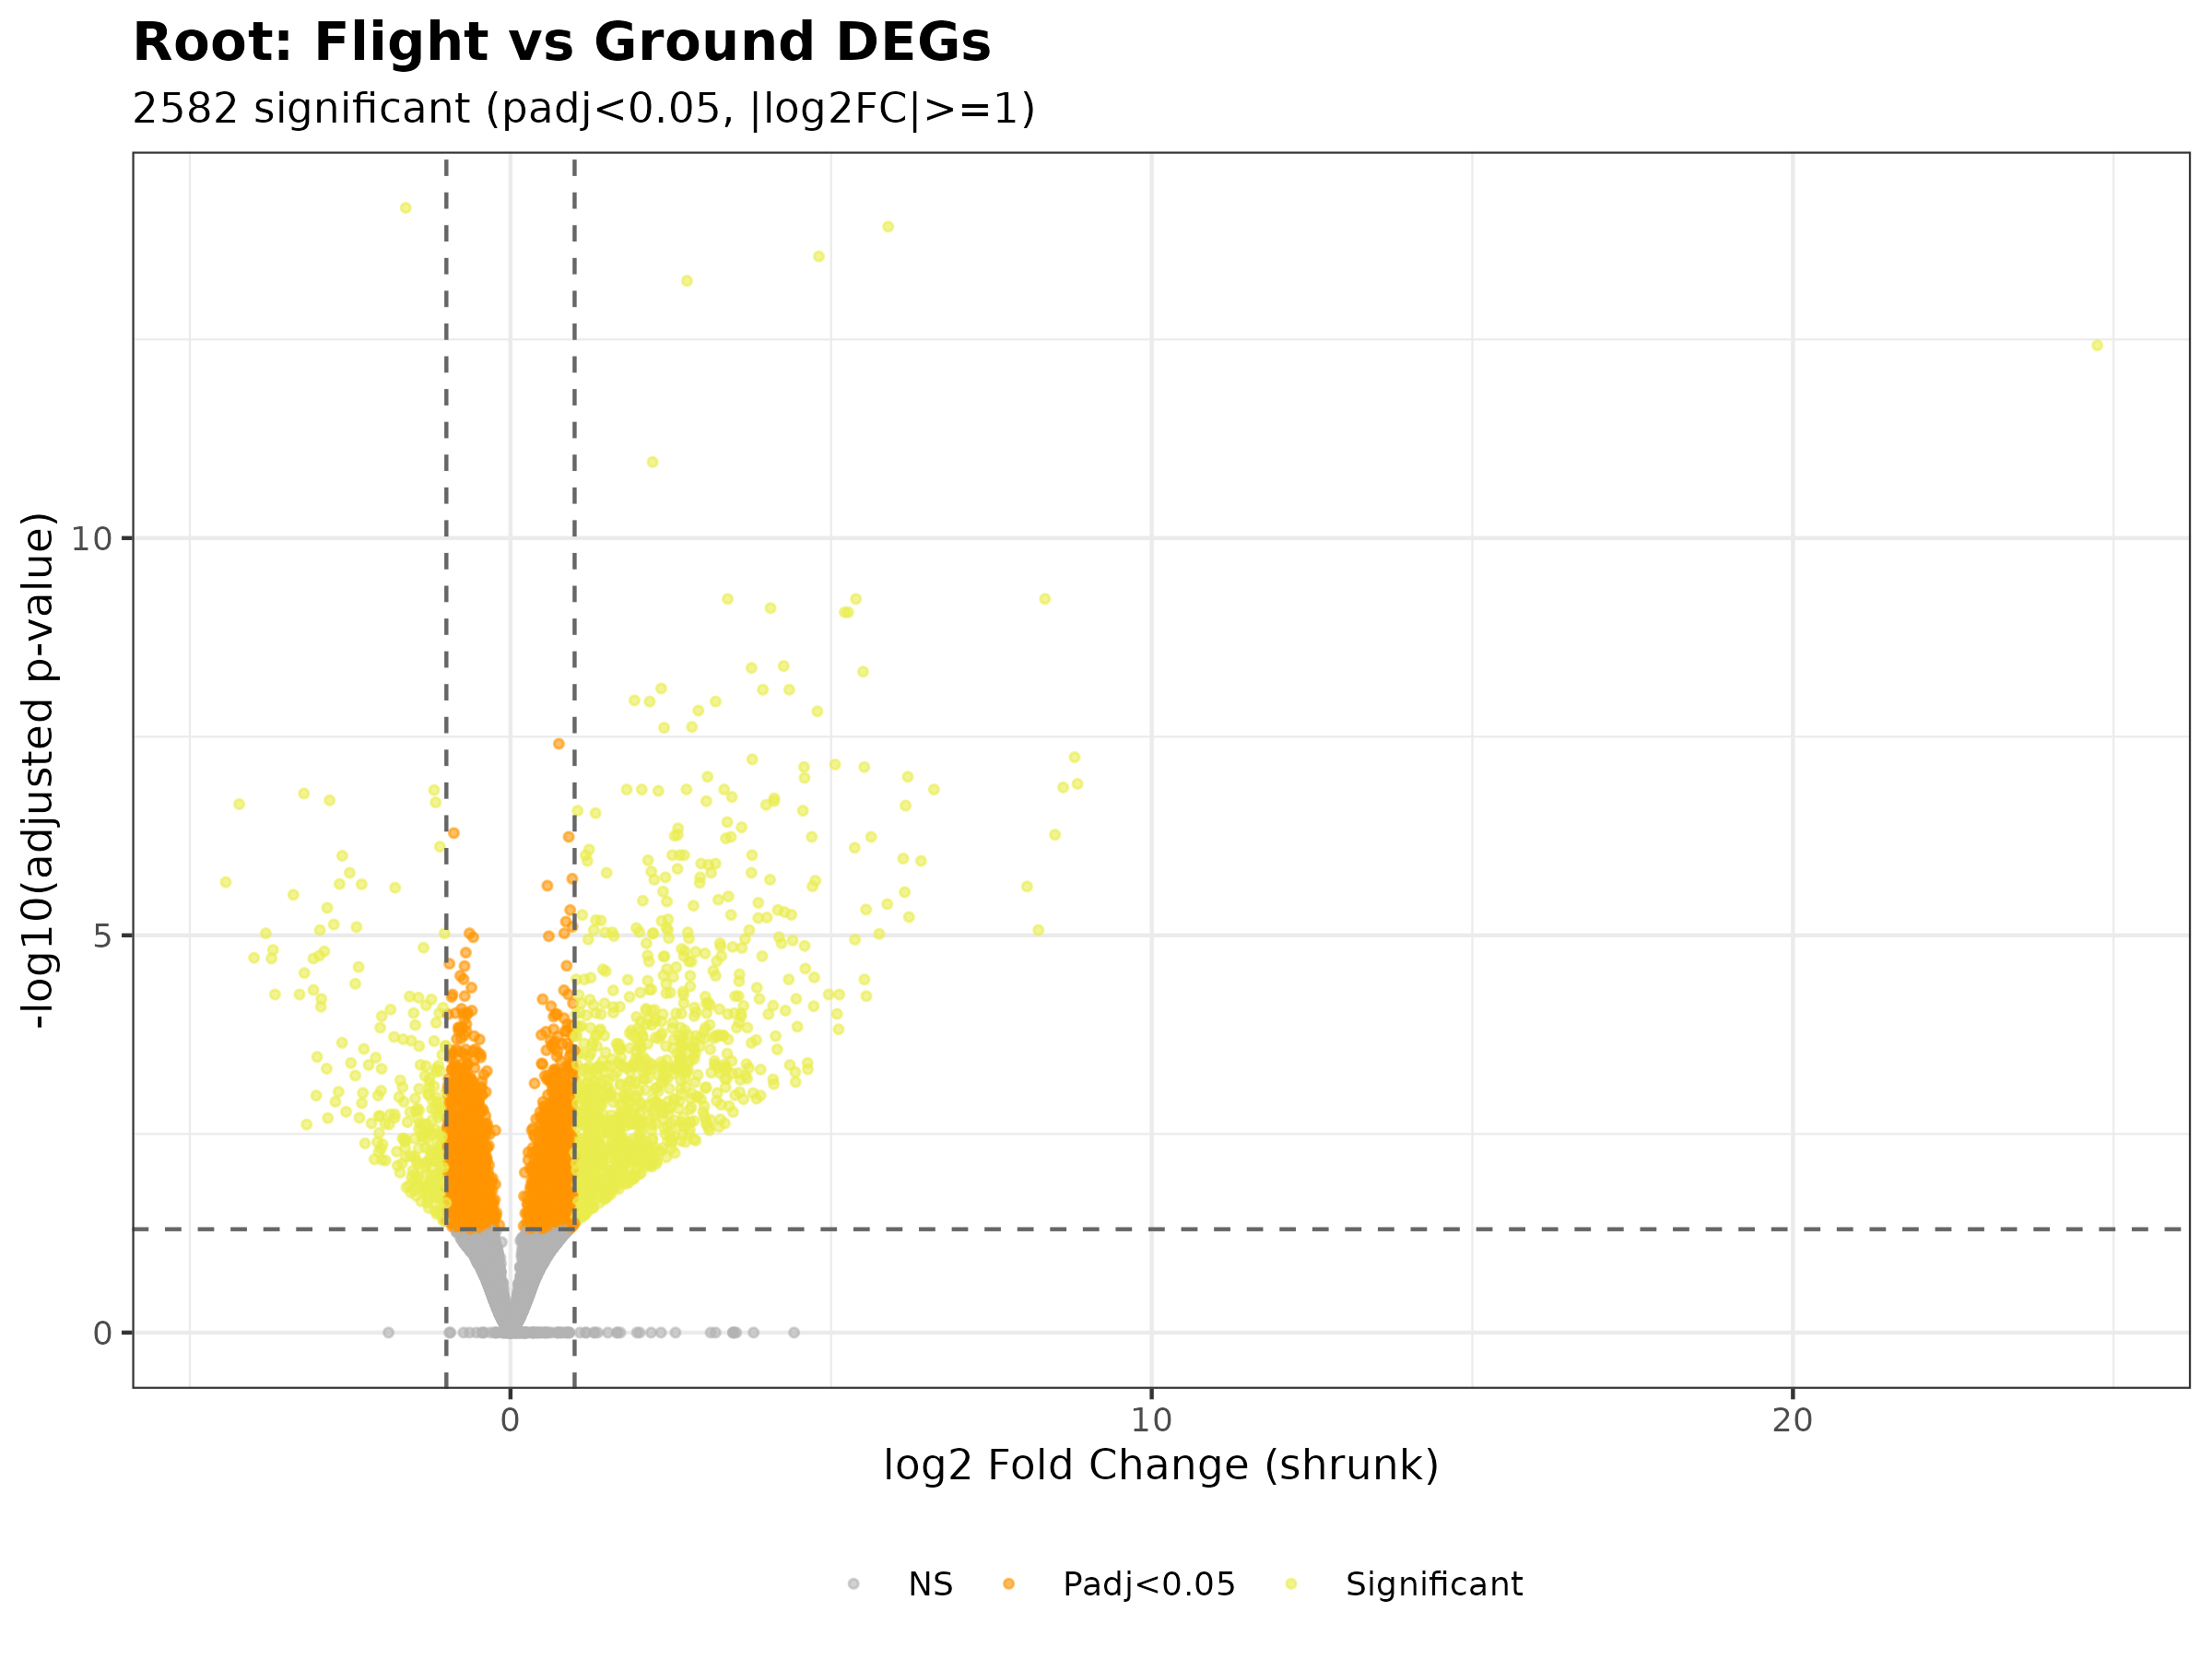
\includegraphics[width=\linewidth]{fig3a_root_volcano.png}\caption{}\end{subfigure}\hfill
\begin{subfigure}{0.46\textwidth}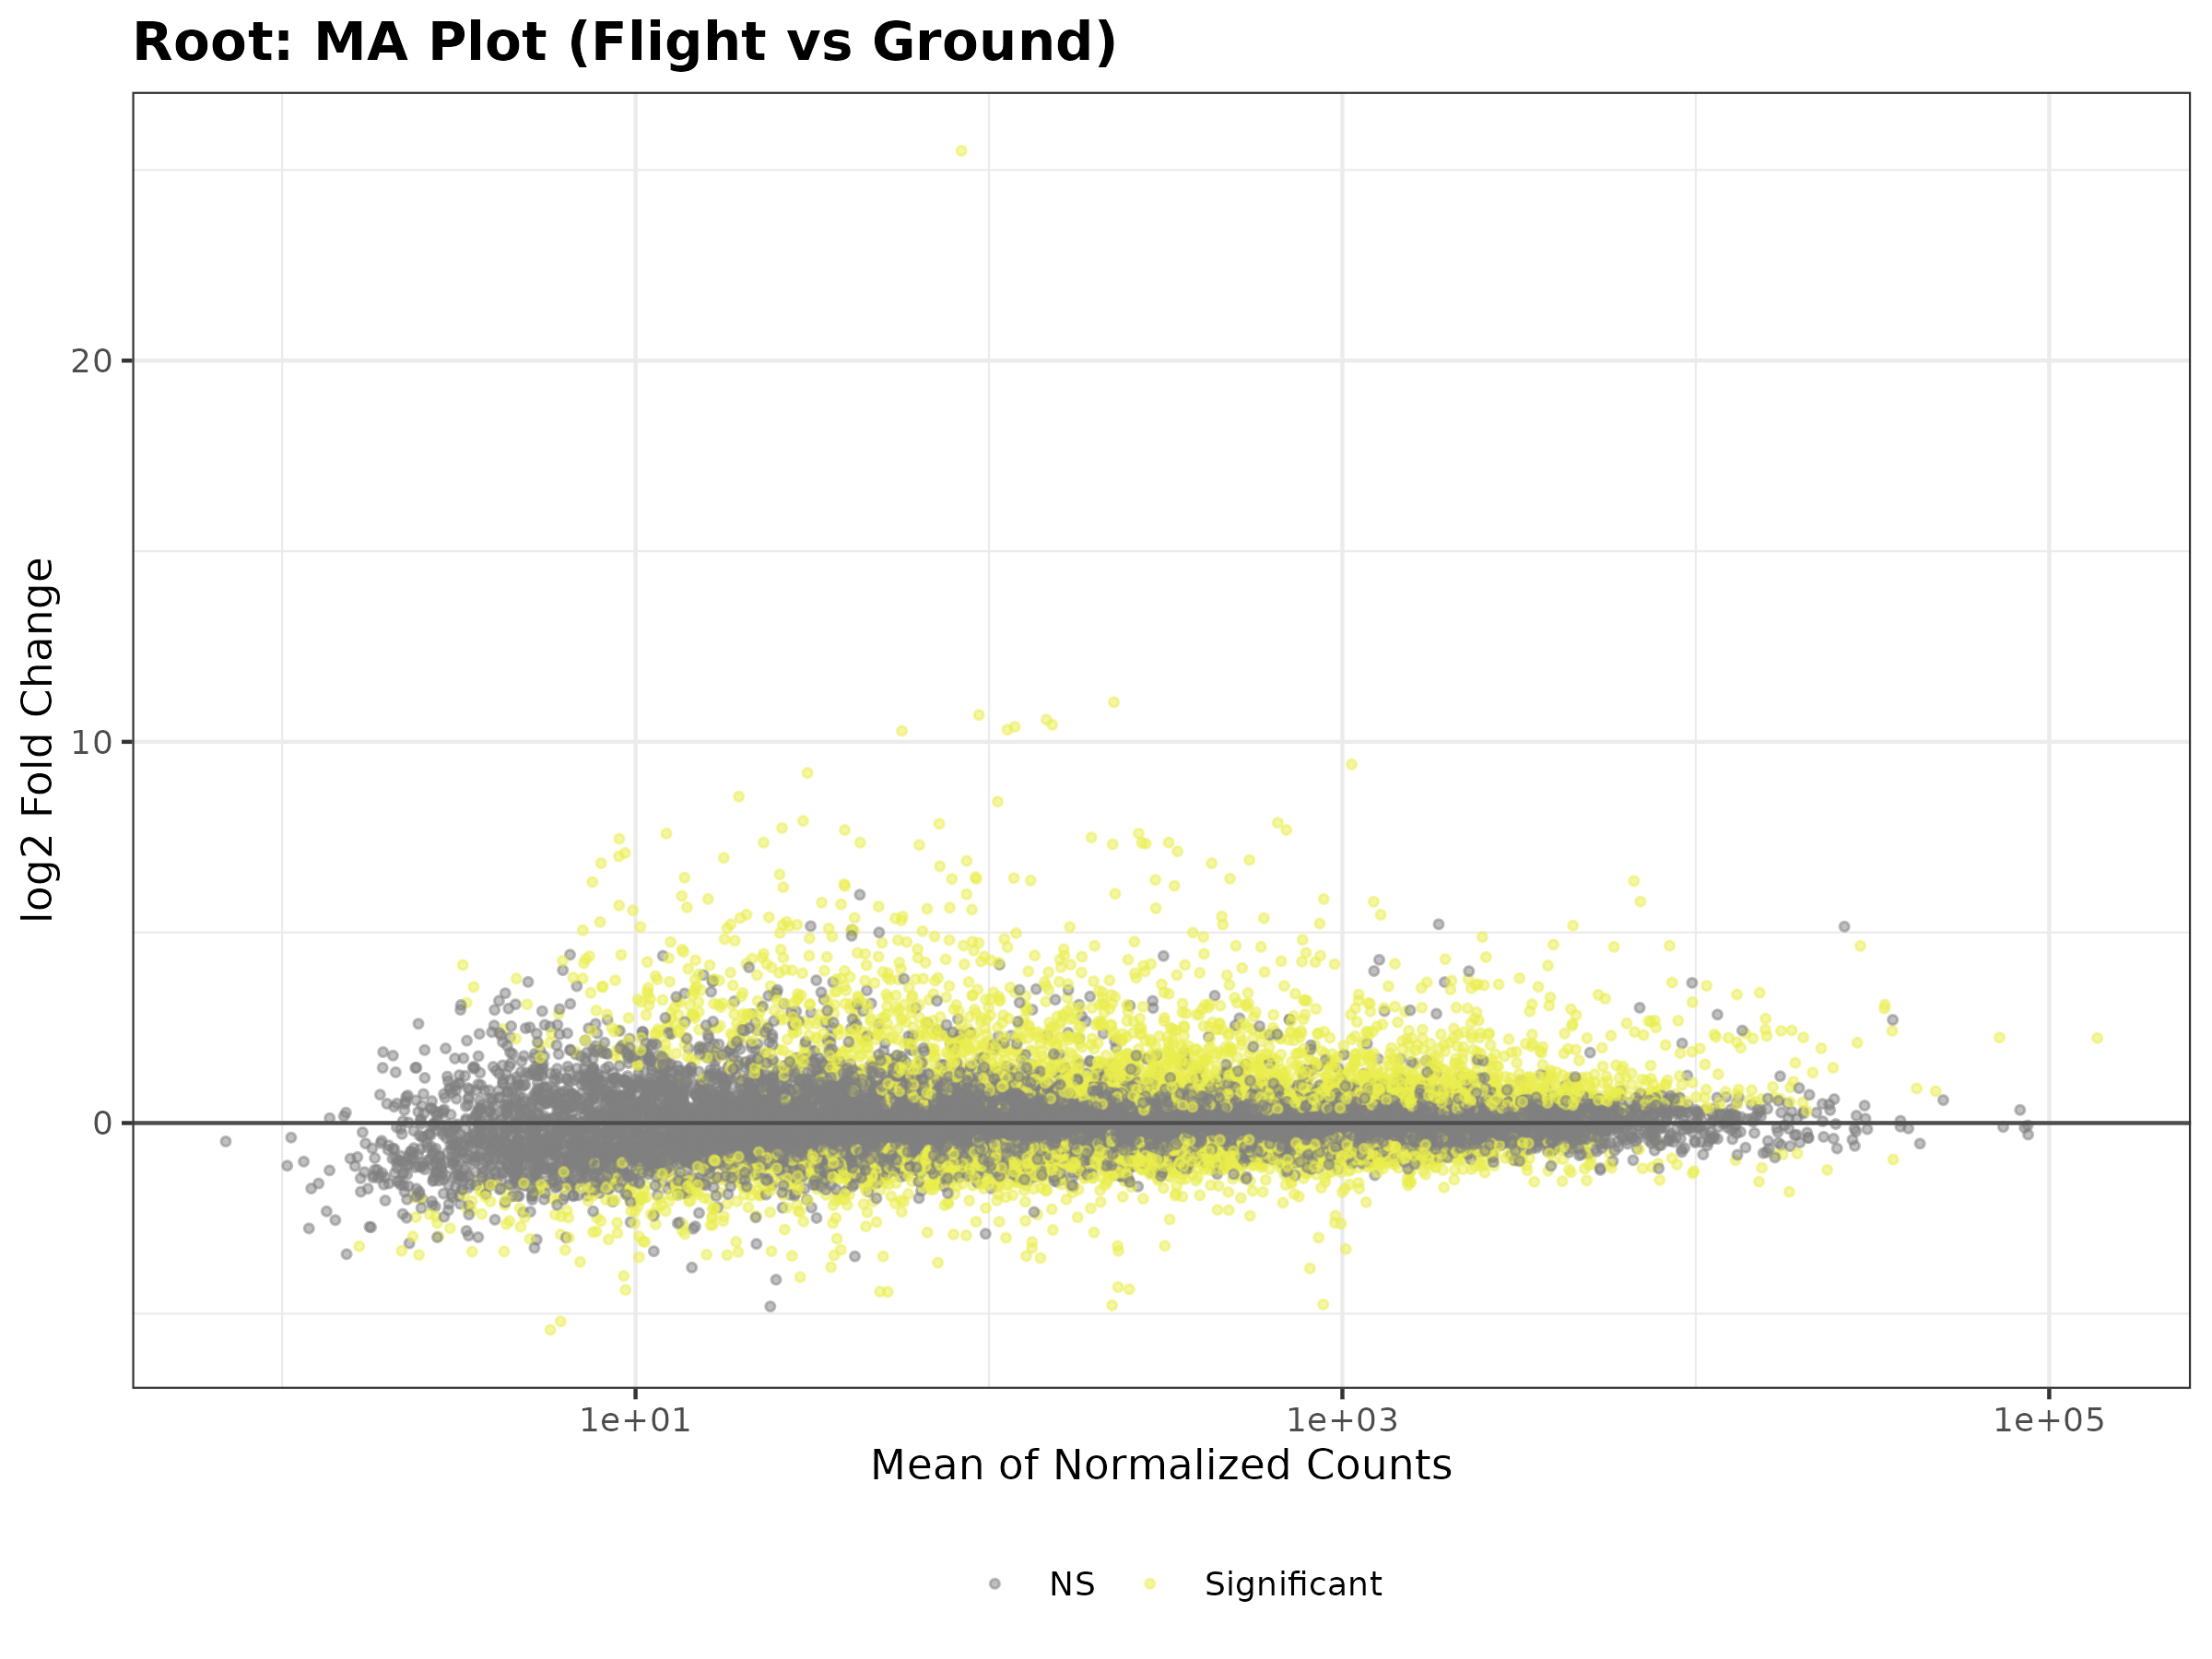
\includegraphics[width=\linewidth]{fig3b_root_ma.png}\caption{}\end{subfigure}
\caption{\textbf{Adventitious roots show a larger, up-regulation-biased response.}
(\textbf{a})~Volcano and (\textbf{b})~MA plots of the root Flight-versus-Ground
contrast. Of 2,582 significant DEGs, 1,706 are up- versus 876 down-regulated
($\approx$2:1 induction bias). Root effect sizes exceed those of leaf, including
switch-like induction of loci from near-zero ground baselines (strongest
$\log_2\text{FC}\approx +25$).}
\label{fig:root}
\end{figure*}

\begin{figure*}[t]
\centering
\begin{subfigure}{0.33\textwidth}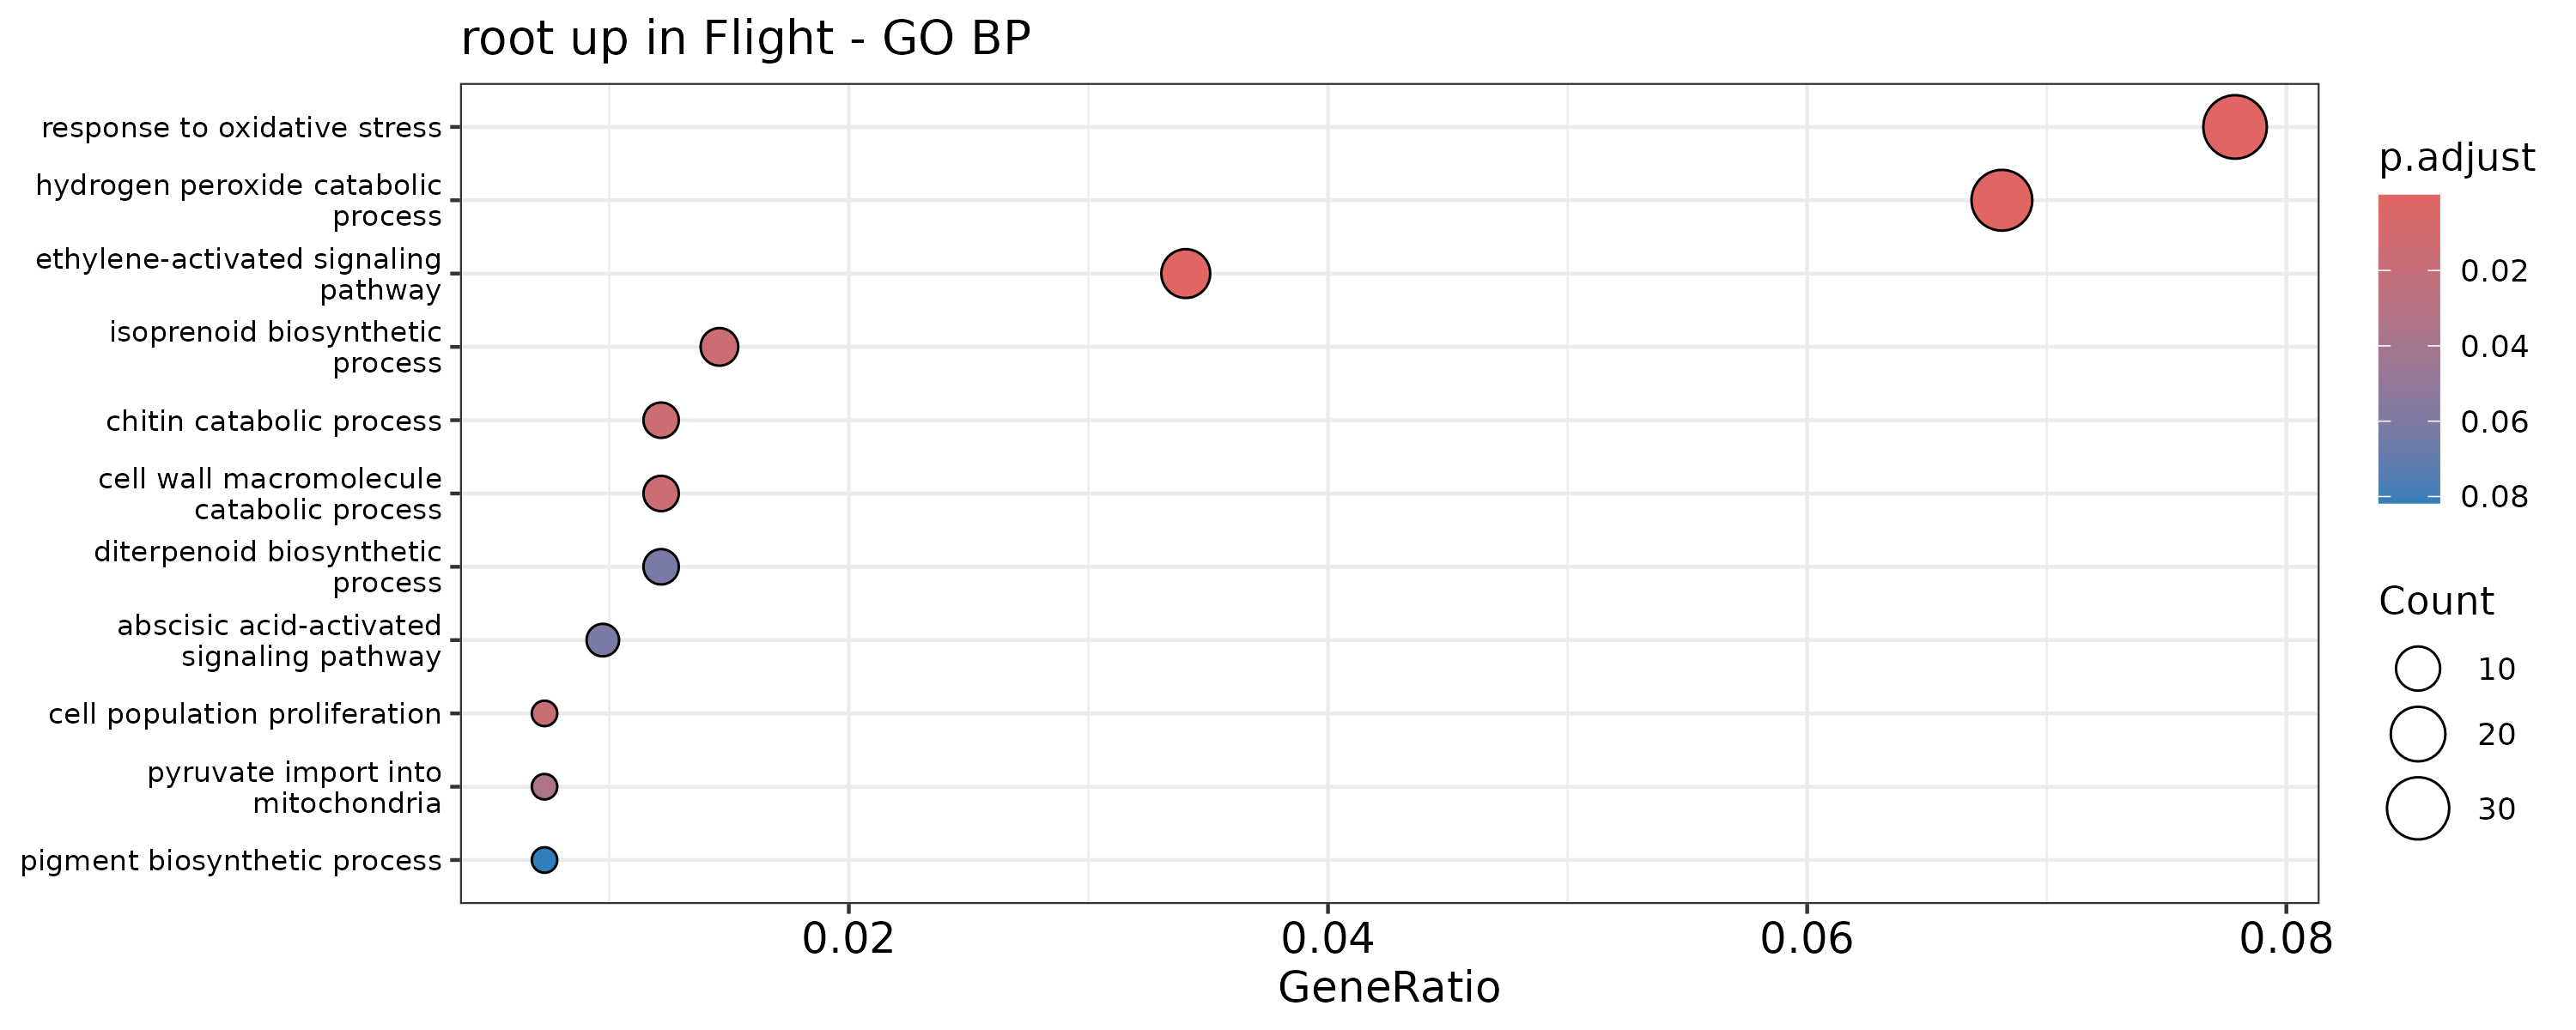
\includegraphics[width=\linewidth]{fig4a_root_go_bp_up.png}\caption{}\end{subfigure}\hfill
\begin{subfigure}{0.33\textwidth}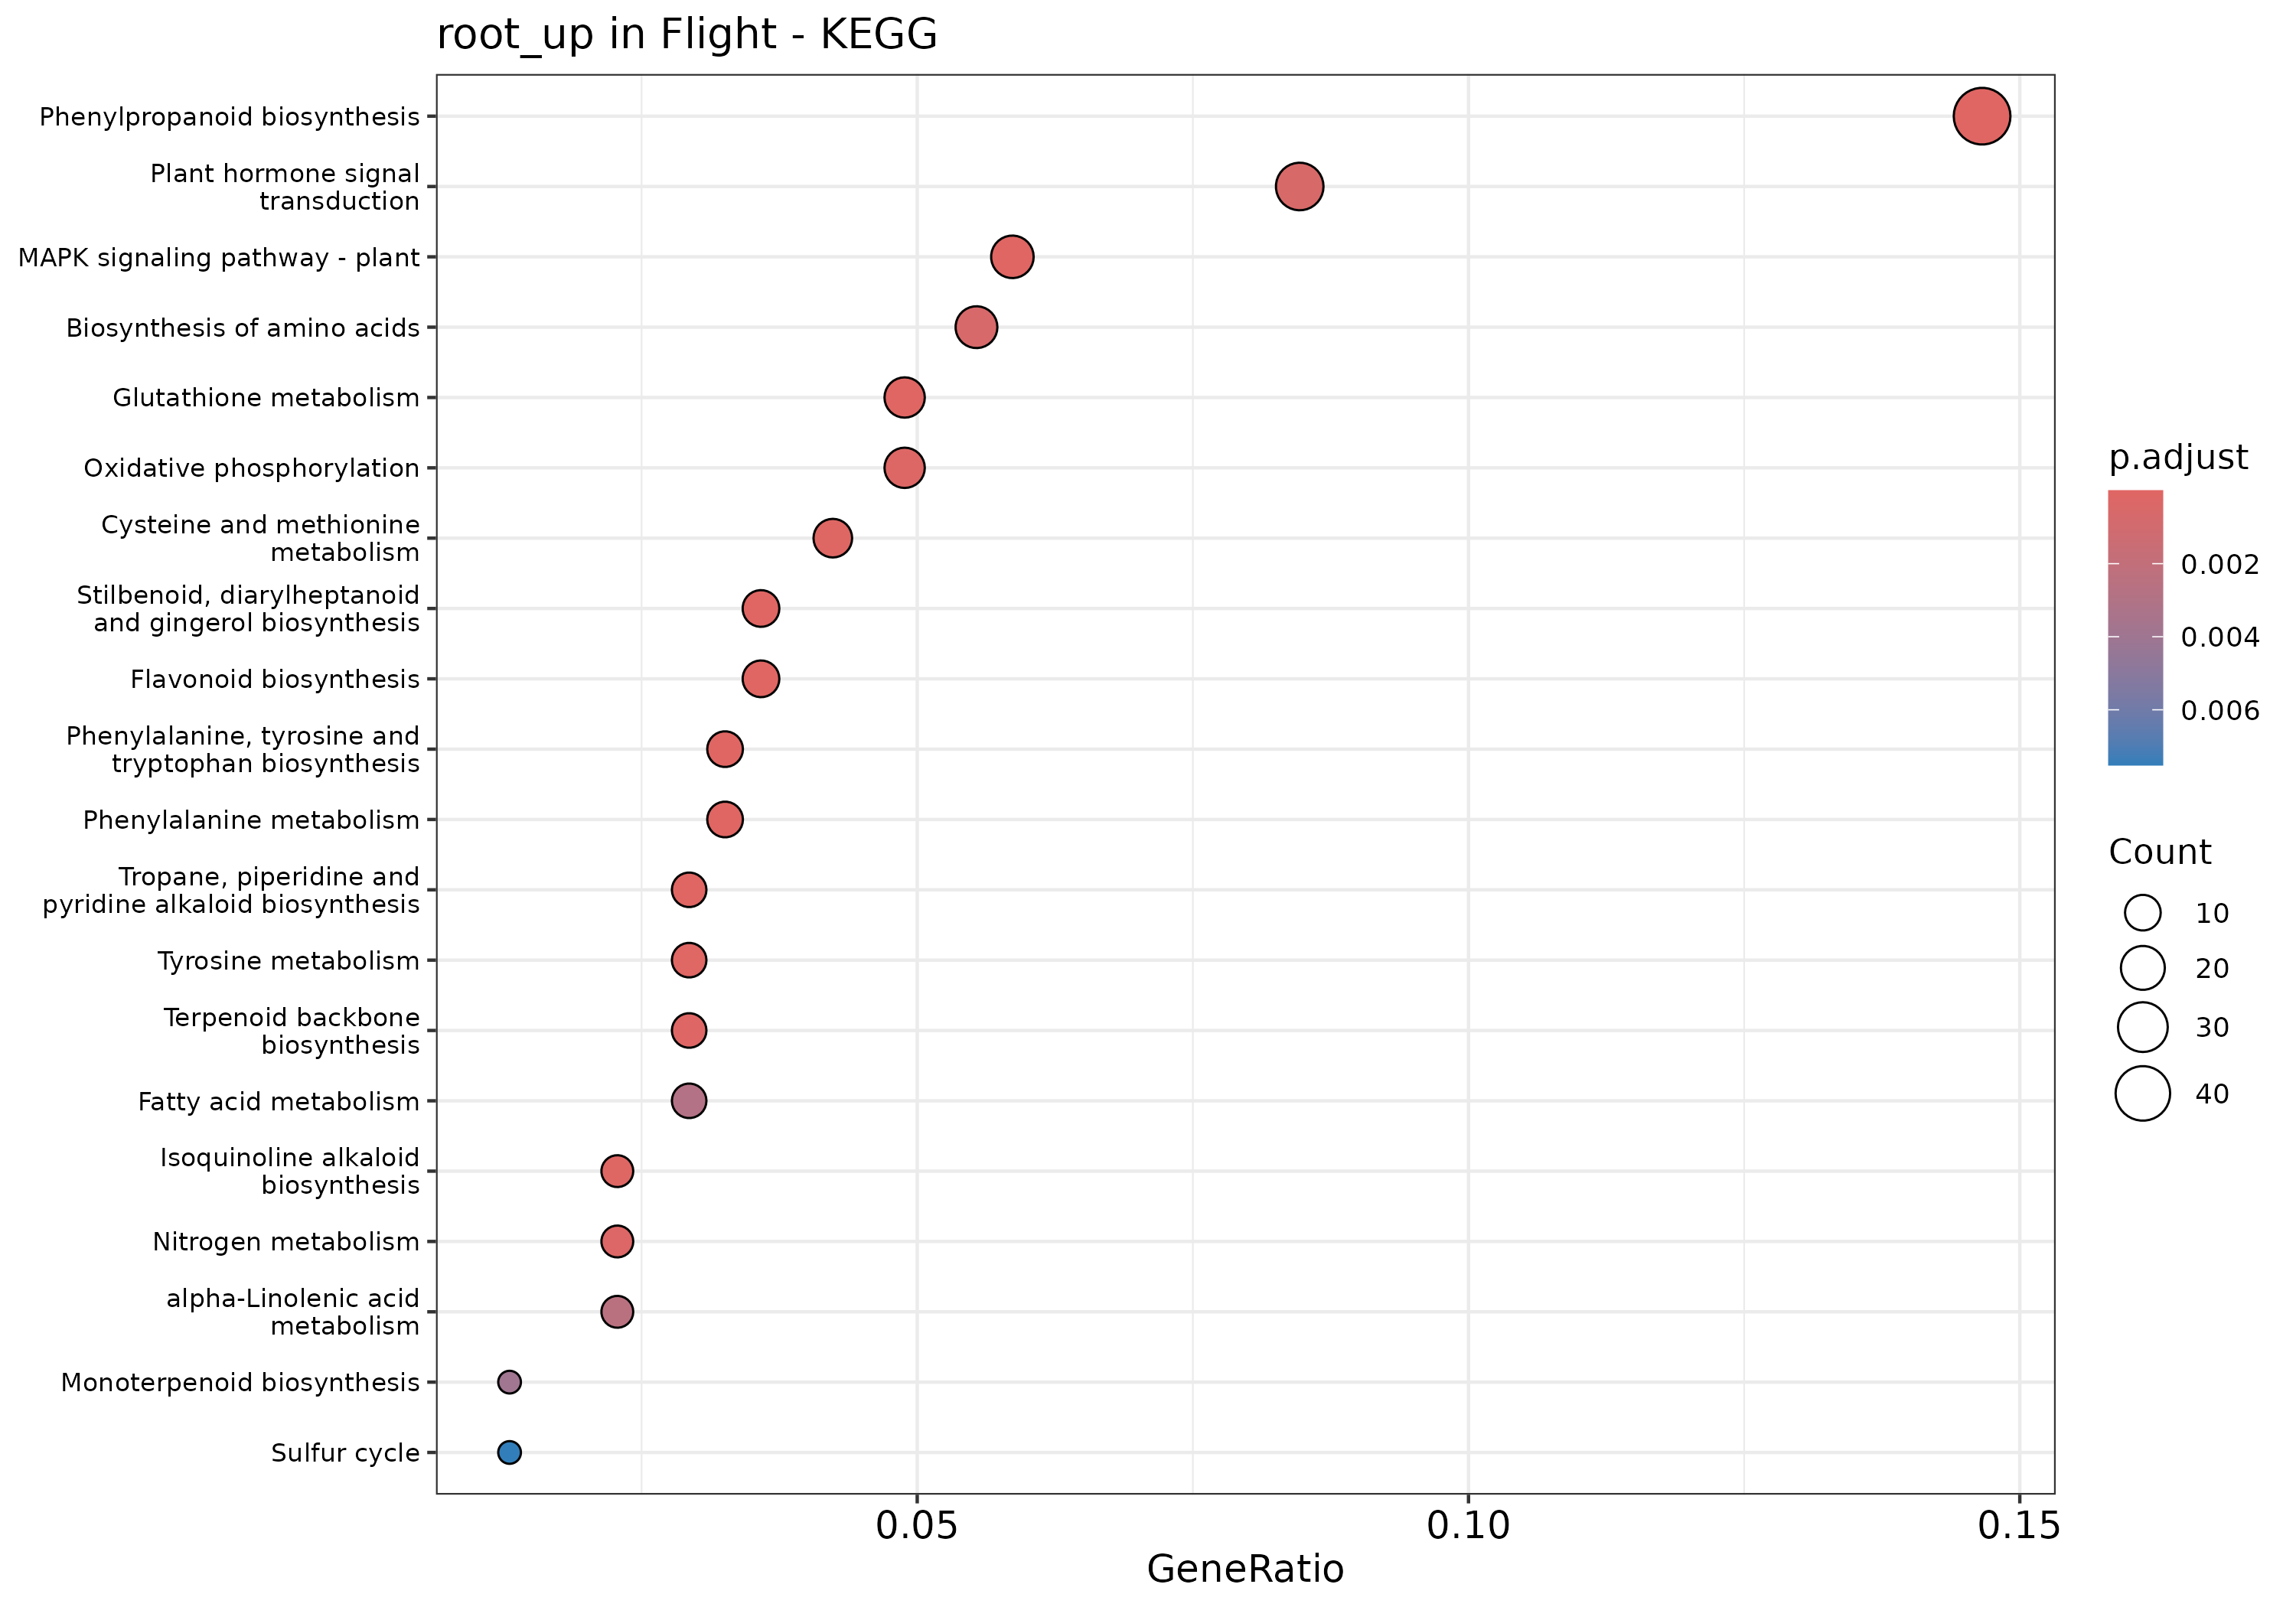
\includegraphics[width=\linewidth]{fig4b_root_kegg_up.png}\caption{}\end{subfigure}\hfill
\begin{subfigure}{0.33\textwidth}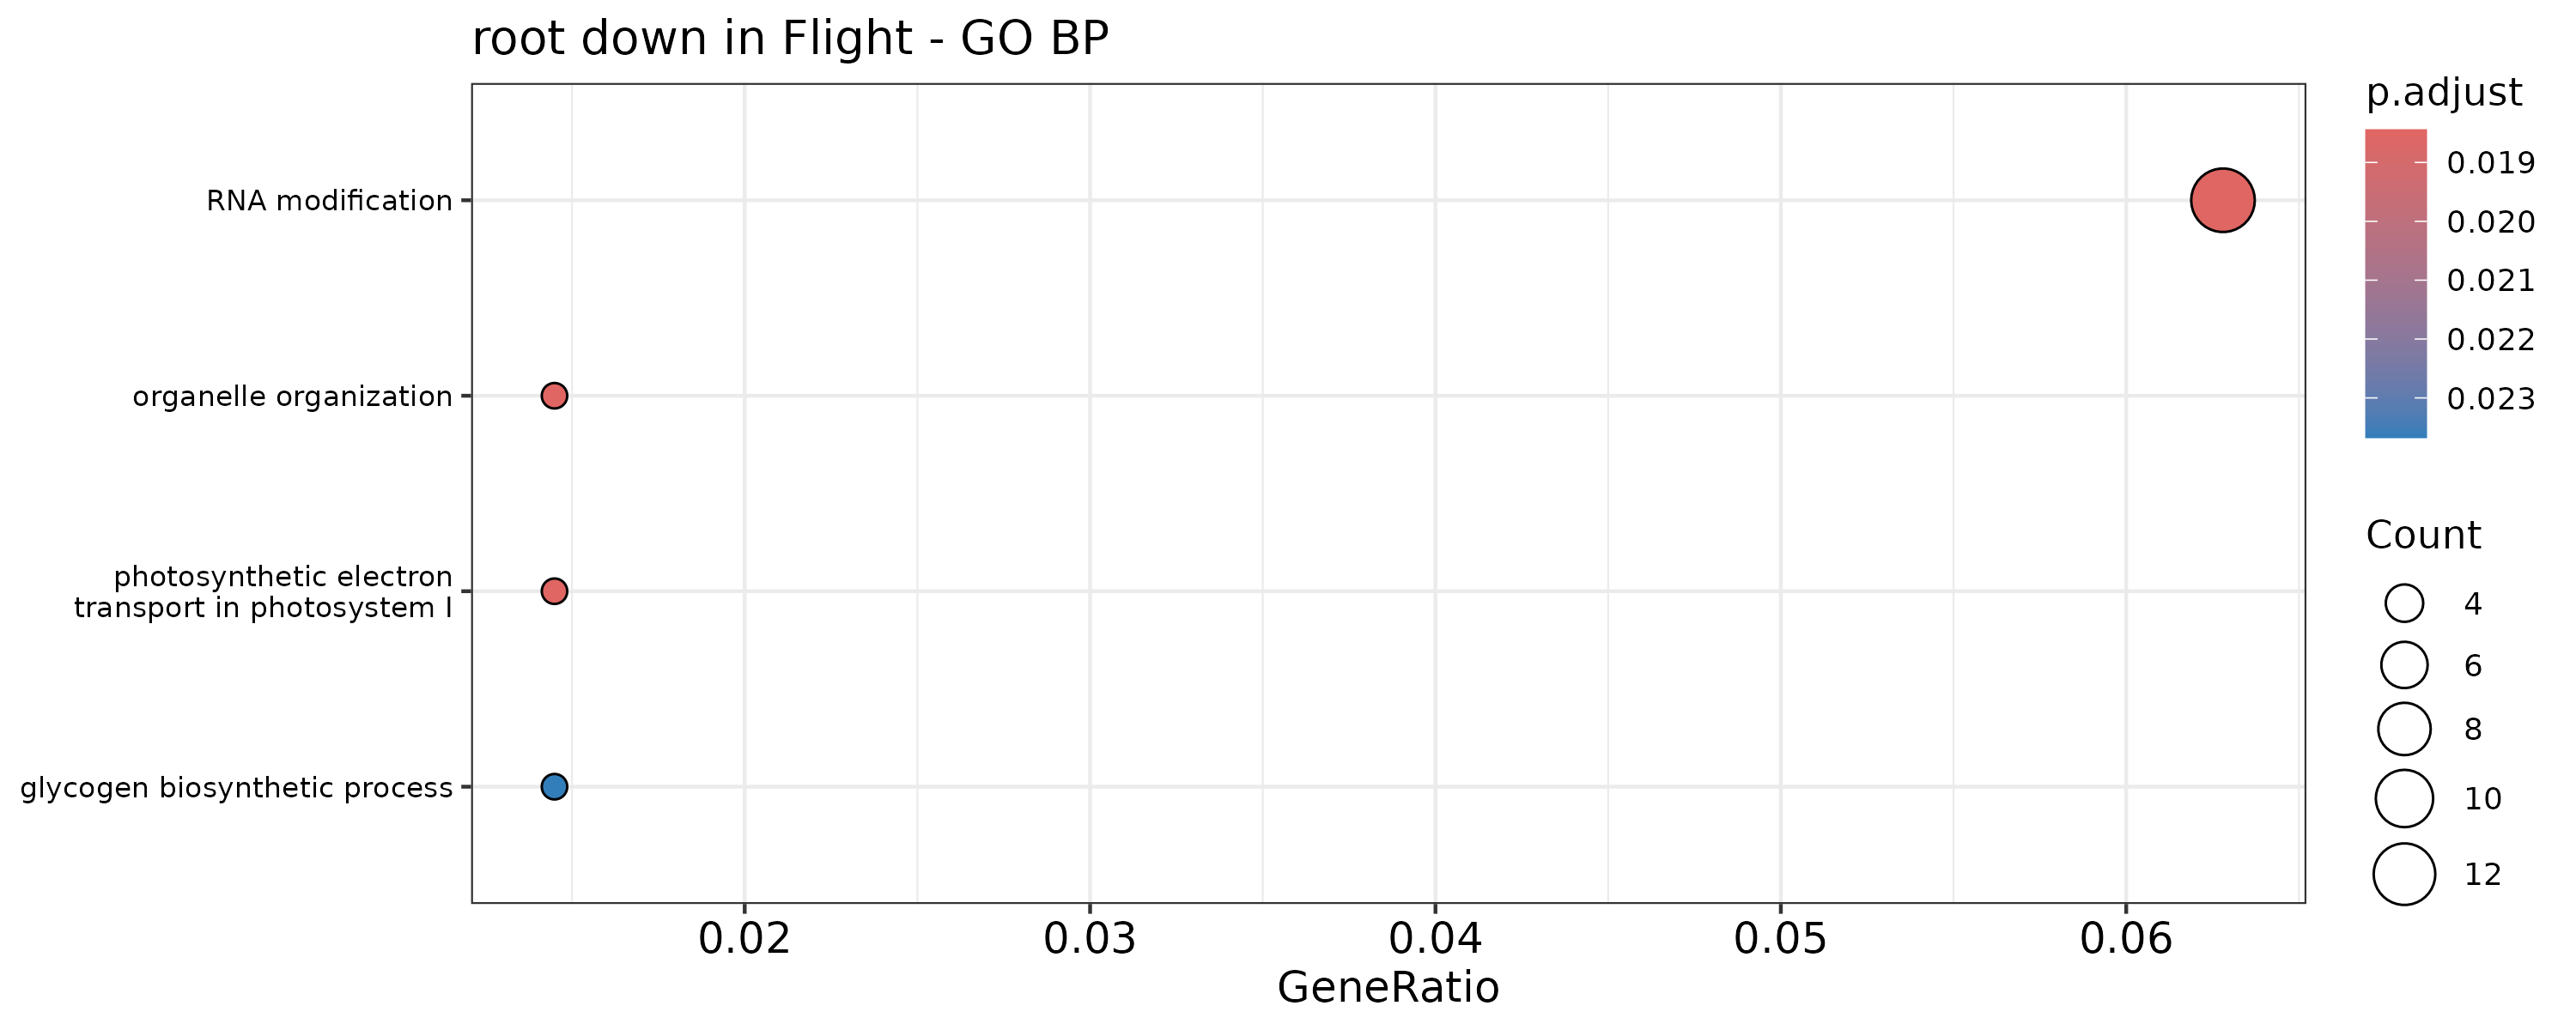
\includegraphics[width=\linewidth]{fig4c_root_go_bp_down.png}\caption{}\end{subfigure}
\caption{\textbf{Root functional enrichment centres on oxidative-stress management and
phenylpropanoid metabolism.} Dot plots (dot size, gene count; colour, adjusted $p$;
$x$-axis, gene ratio) for root DEGs. (\textbf{a})~GO biological process, up-regulated:
led by response to oxidative stress and hydrogen-peroxide catabolism. (\textbf{b})~KEGG,
up-regulated: dominated by phenylpropanoid biosynthesis (FDR $\approx 4\times10^{-30}$),
with flavonoid/stilbenoid biosynthesis, glutathione metabolism and plant-hormone
signalling. (\textbf{c})~GO biological process, down-regulated.}
\label{fig:enr_root}
\end{figure*}

\begin{figure*}[t]
\centering
\begin{subfigure}{0.33\textwidth}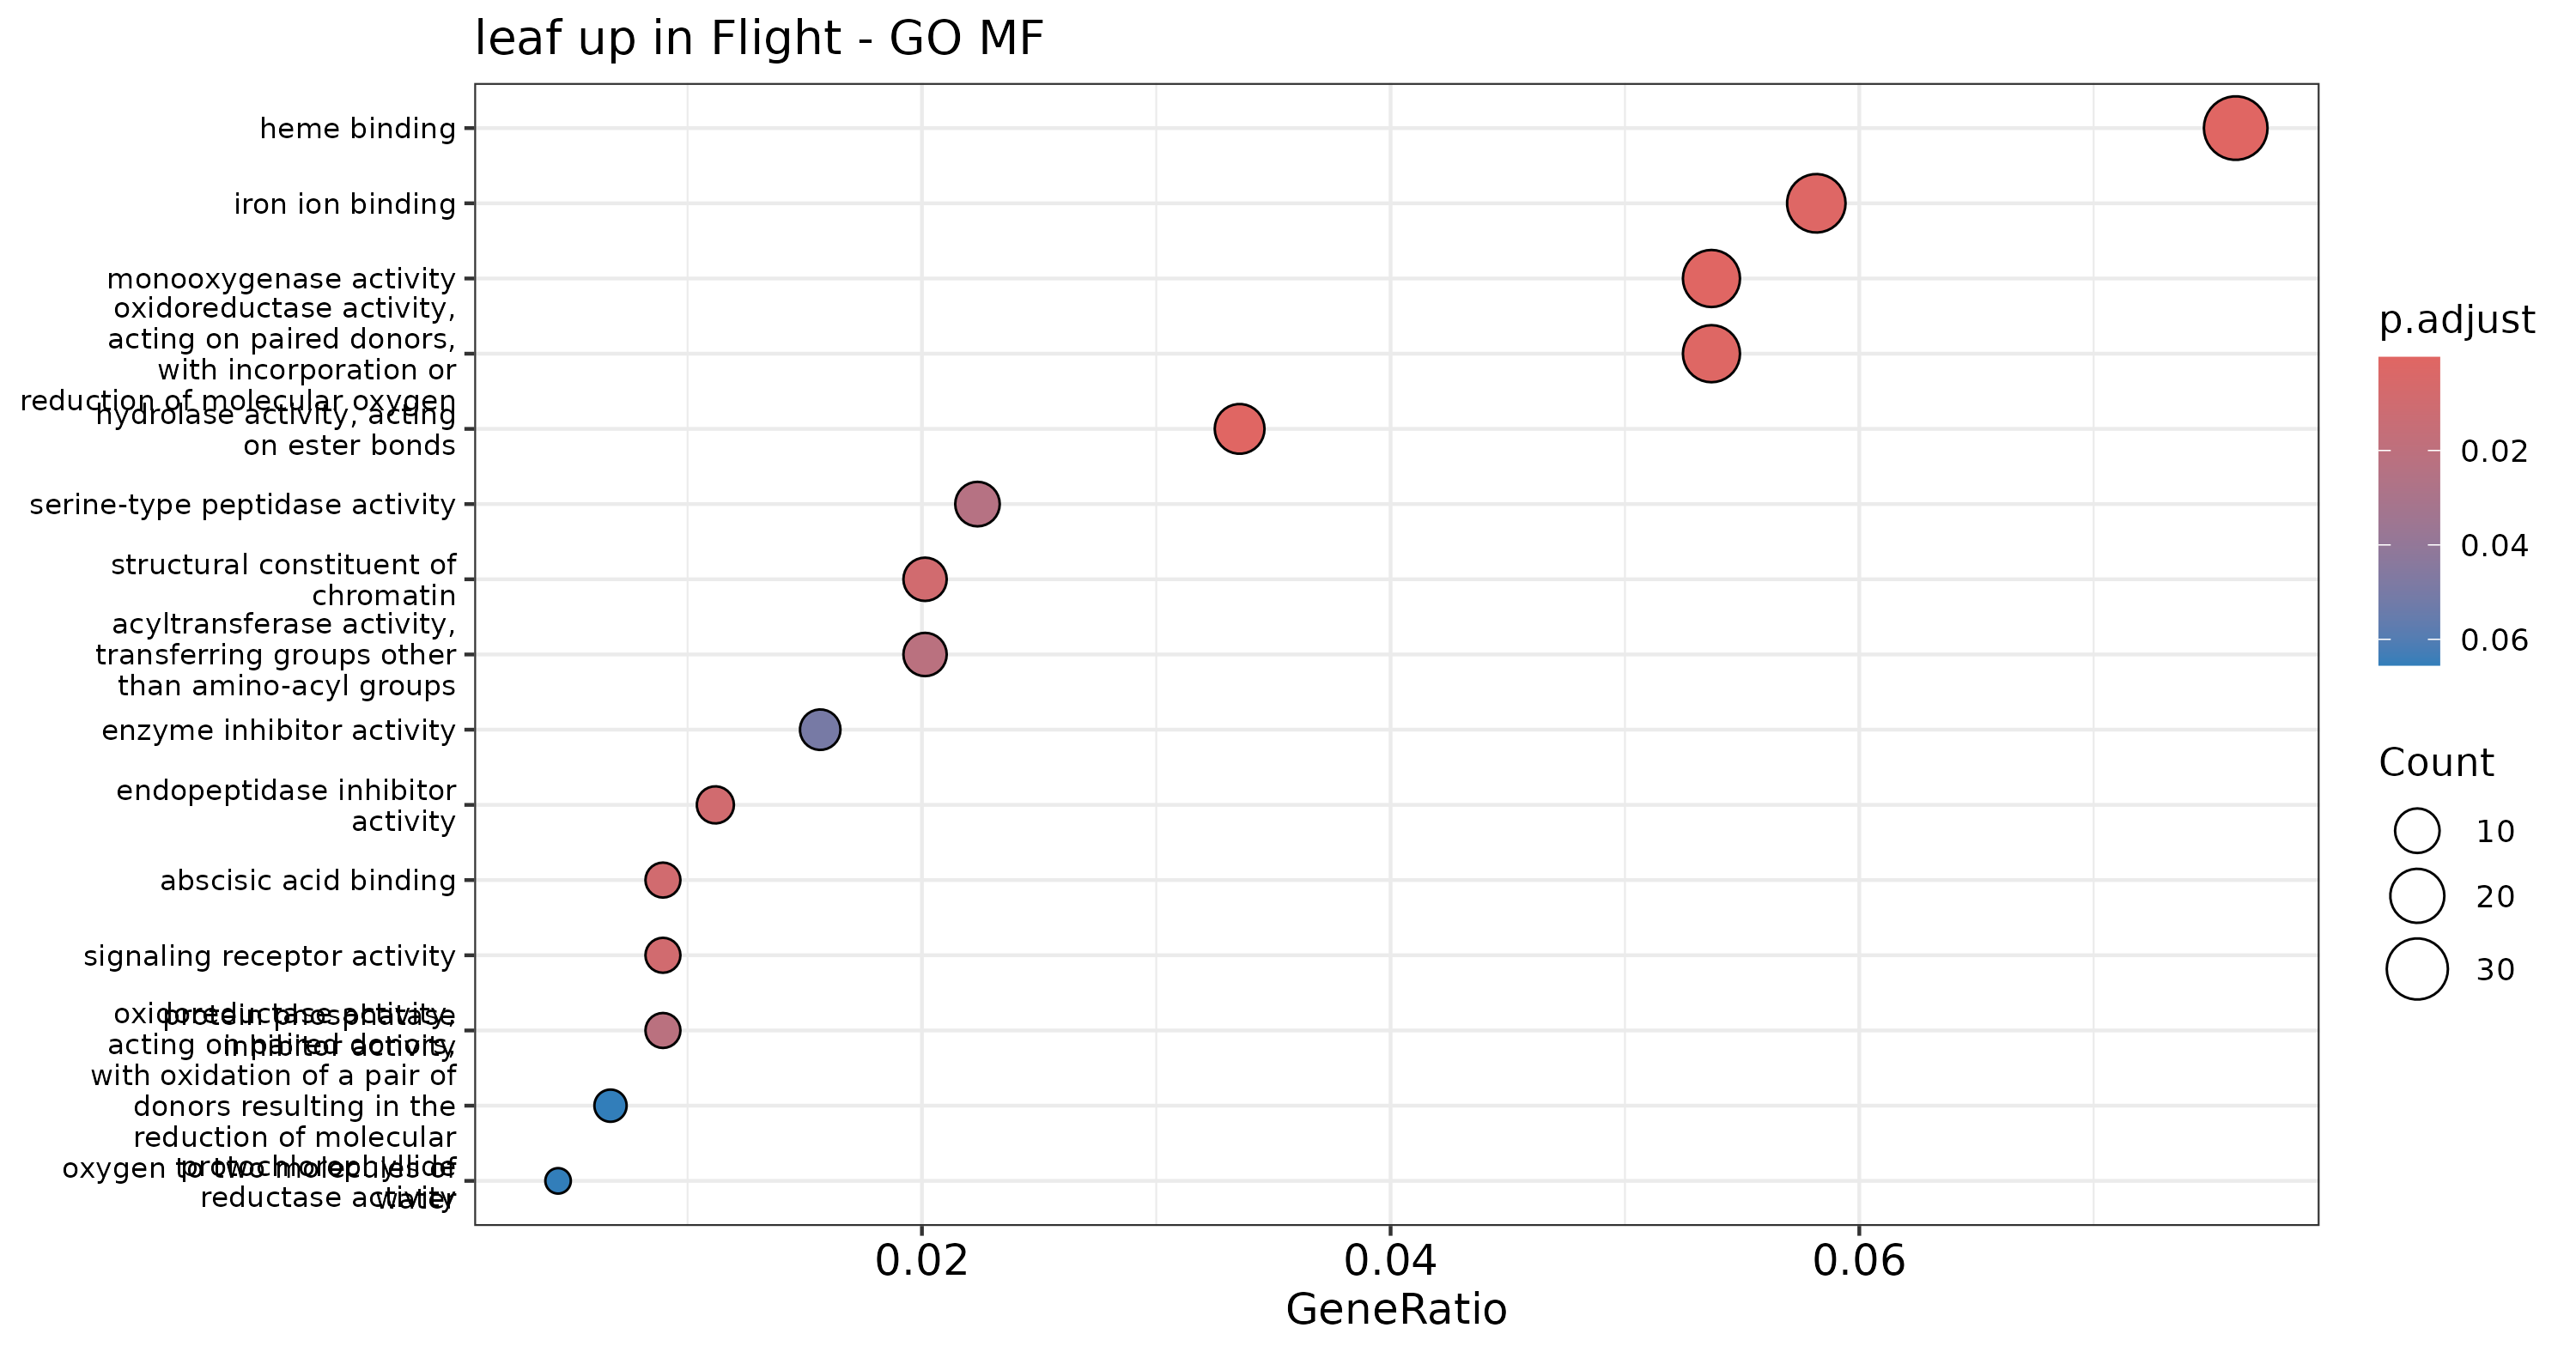
\includegraphics[width=\linewidth]{fig5a_leaf_go_mf_up.png}\caption{}\end{subfigure}\hfill
\begin{subfigure}{0.33\textwidth}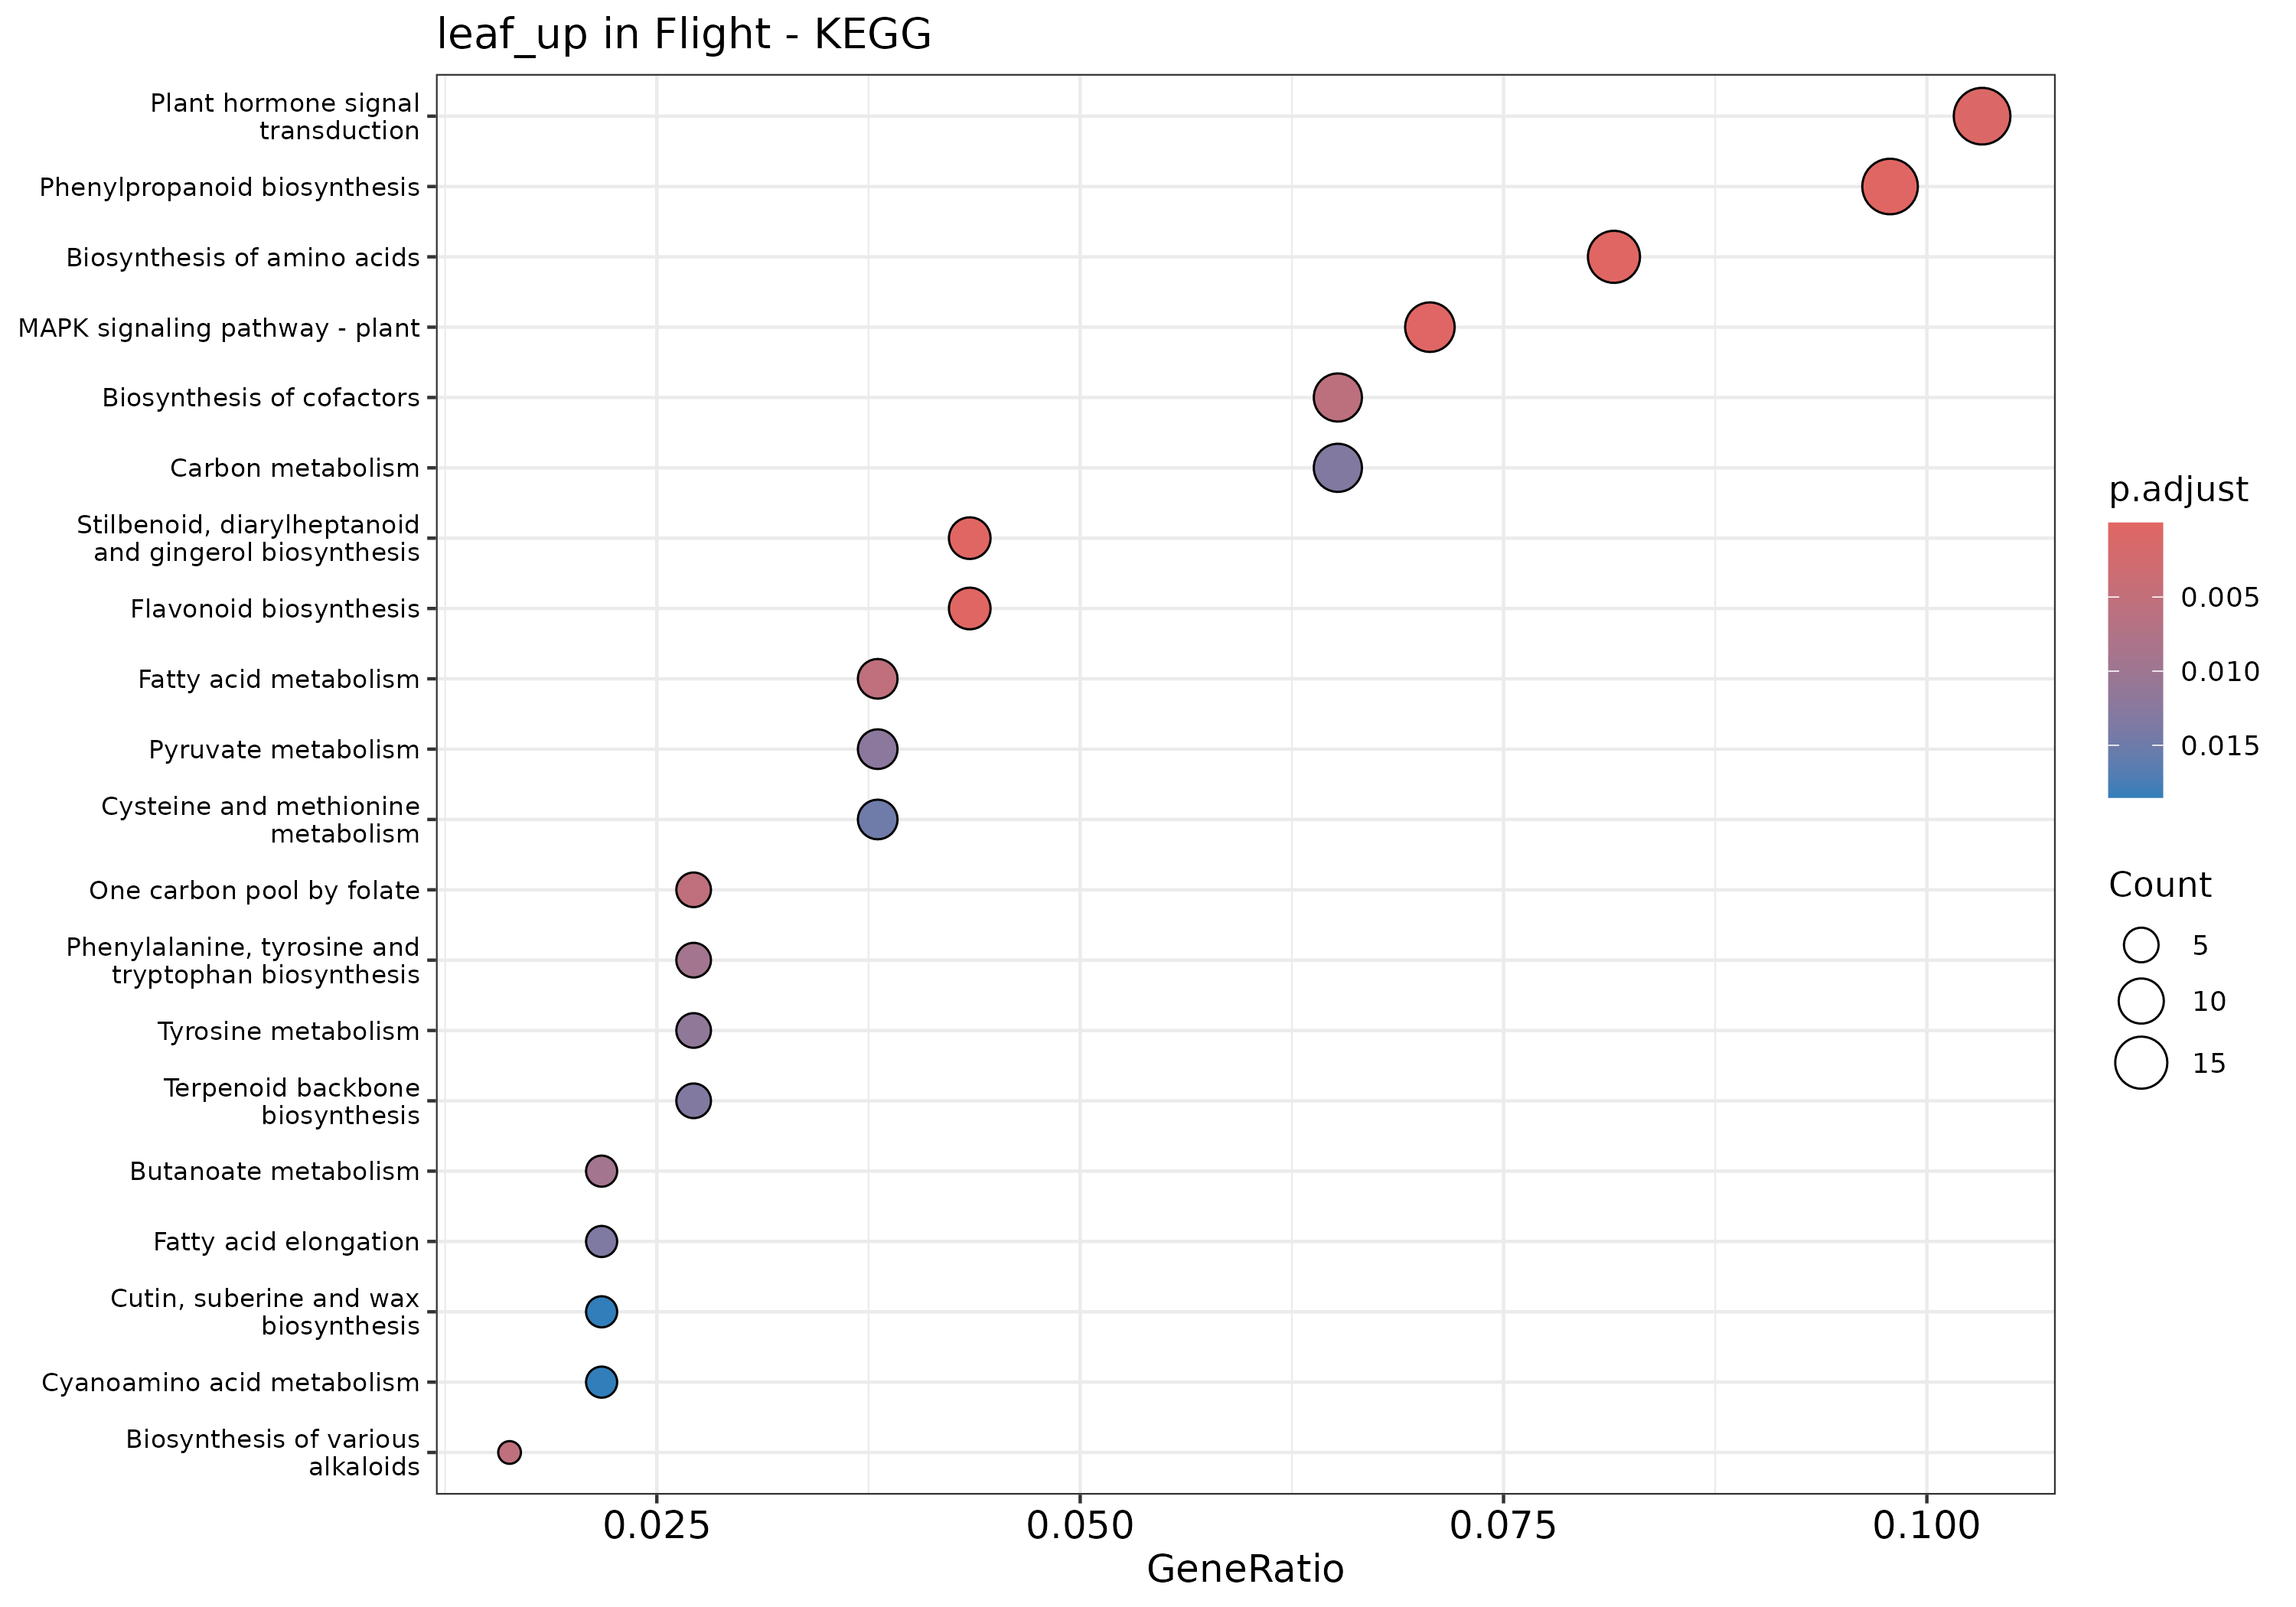
\includegraphics[width=\linewidth]{fig5b_leaf_kegg_up.png}\caption{}\end{subfigure}\hfill
\begin{subfigure}{0.33\textwidth}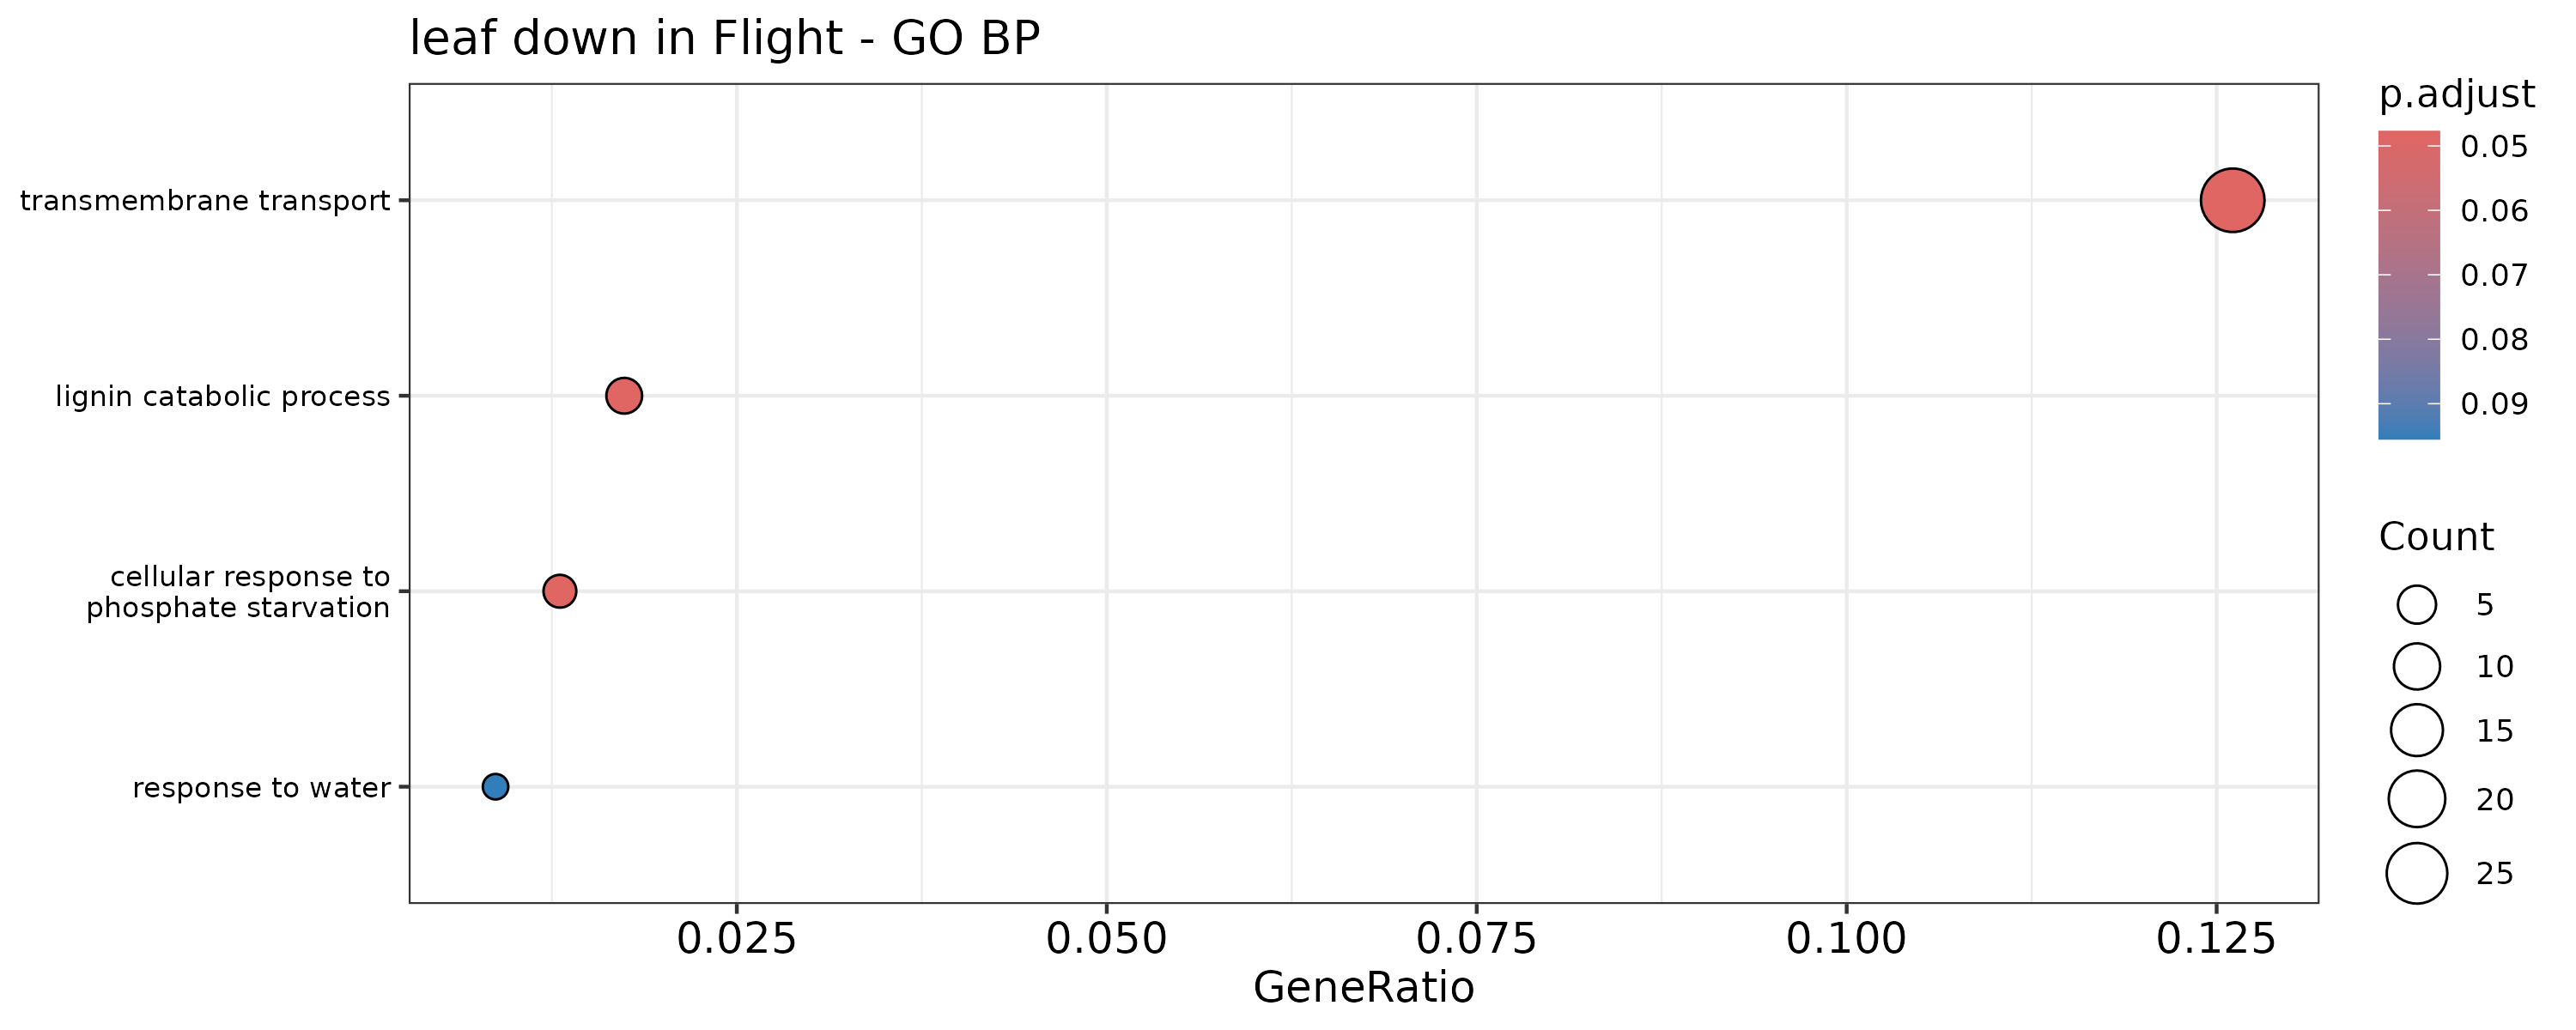
\includegraphics[width=\linewidth]{fig5c_leaf_go_bp_down.png}\caption{}\end{subfigure}
\caption{\textbf{Leaf functional enrichment mirrors the root stress programme.} Dot
plots for leaf DEGs. (\textbf{a})~GO molecular function, up-regulated: heme binding,
monooxygenase/oxidoreductase and iron-ion binding. (\textbf{b})~KEGG, up-regulated:
phenylpropanoid and flavonoid biosynthesis, amino-acid biosynthesis, MAPK signalling
and plant-hormone signal transduction. (\textbf{c})~GO biological process,
down-regulated, including transmembrane transport; the plant circadian-rhythm KEGG
pathway is down-regulated in both organs.}
\label{fig:enr_leaf}
\end{figure*}

\begin{figure*}[t]
\centering
\begin{subfigure}{0.40\textwidth}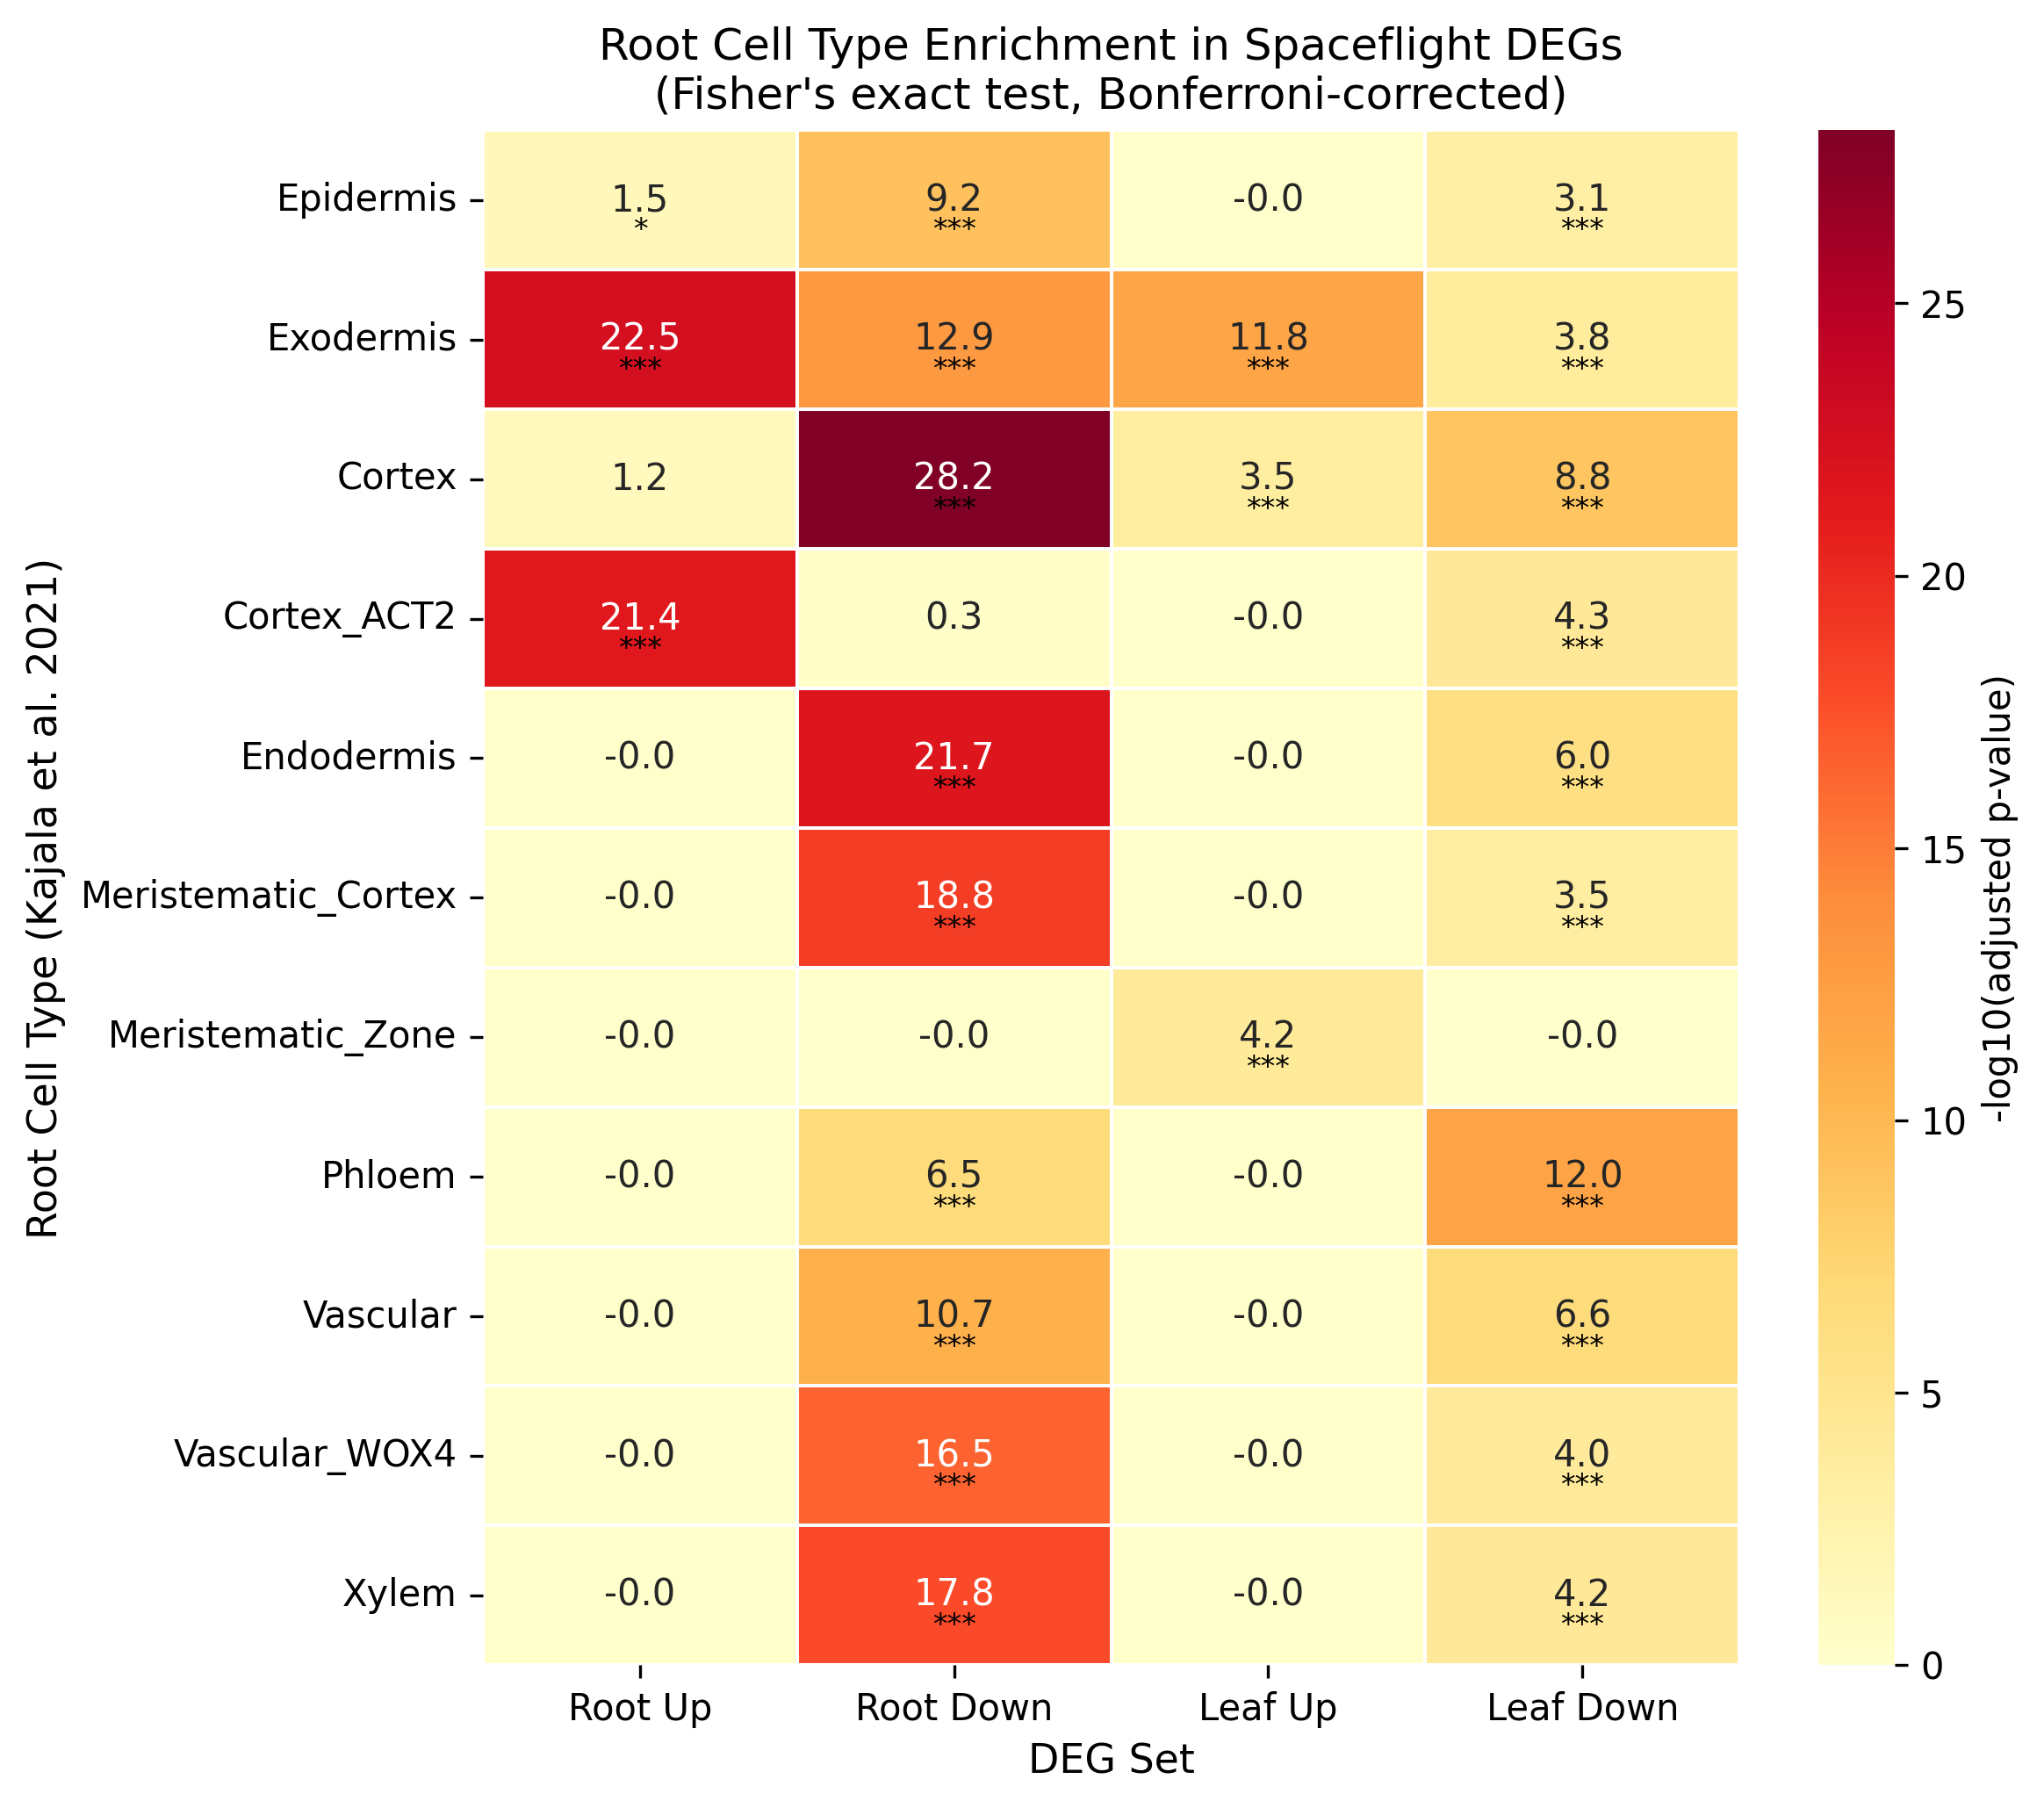
\includegraphics[width=\linewidth]{fig6a_root_celltype_heat.png}\caption{}\end{subfigure}\hfill
\begin{subfigure}{0.28\textwidth}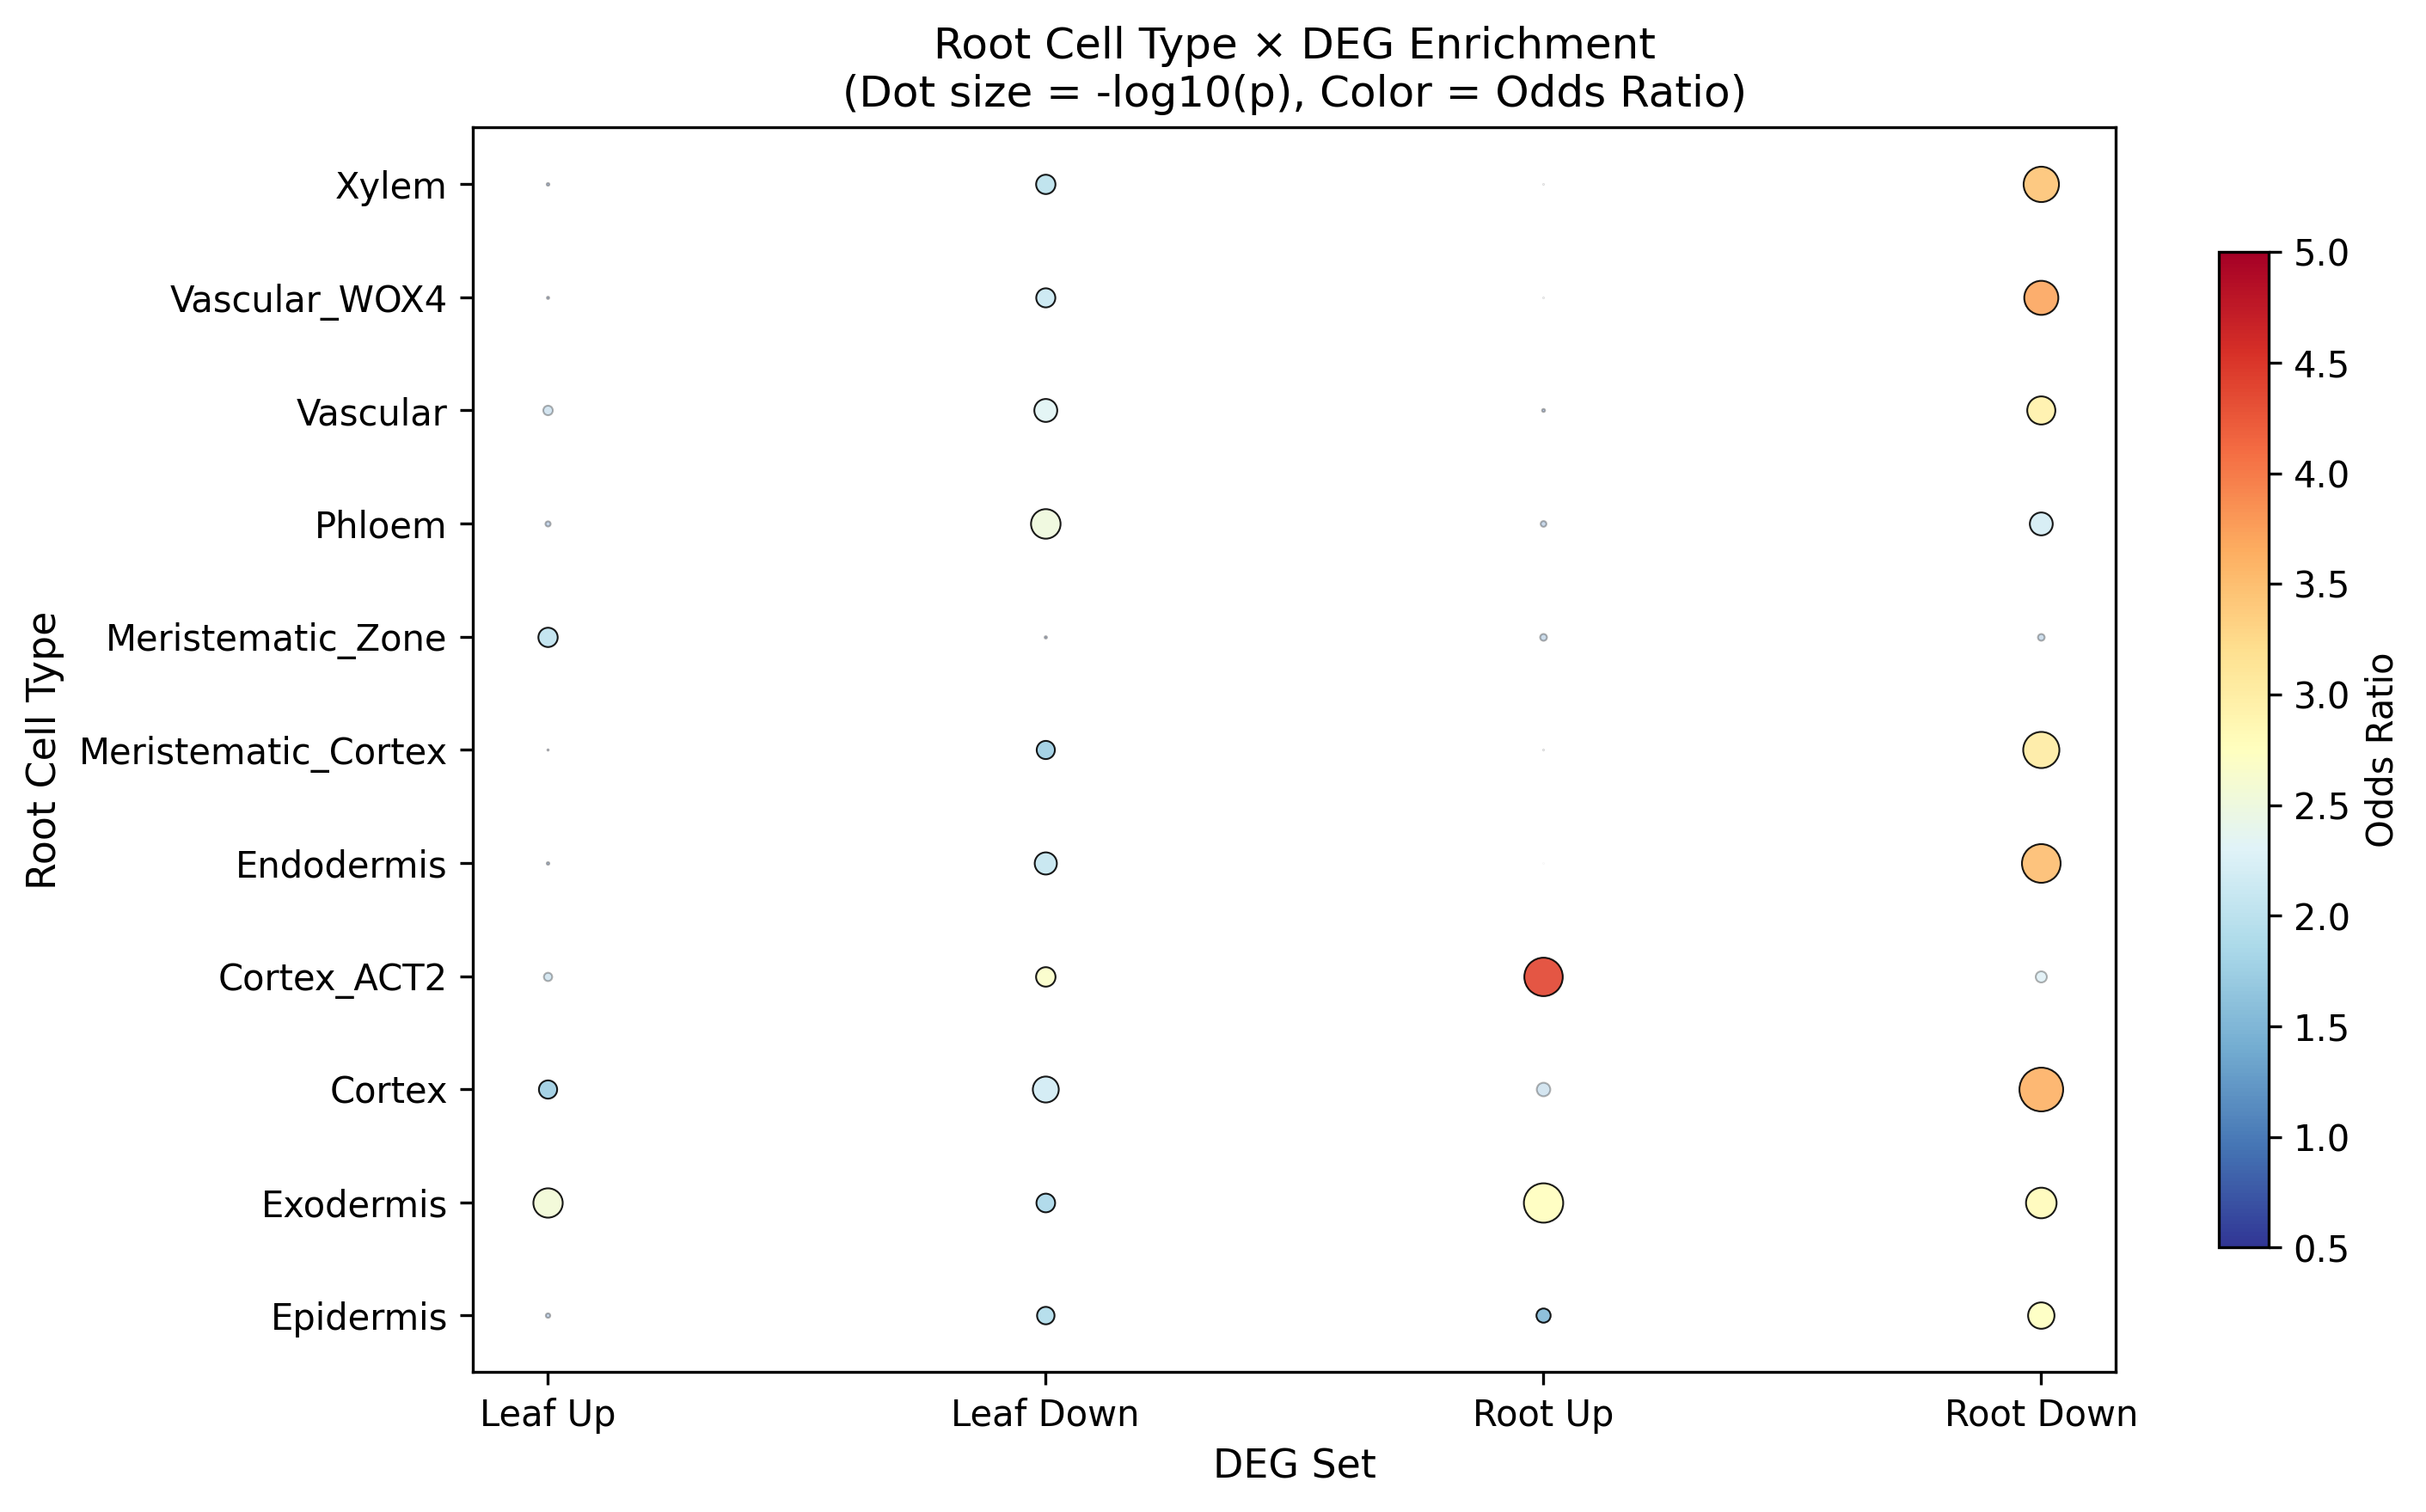
\includegraphics[width=\linewidth]{fig6b_root_celltype_dot.png}\caption{}\end{subfigure}\hfill
\begin{subfigure}{0.28\textwidth}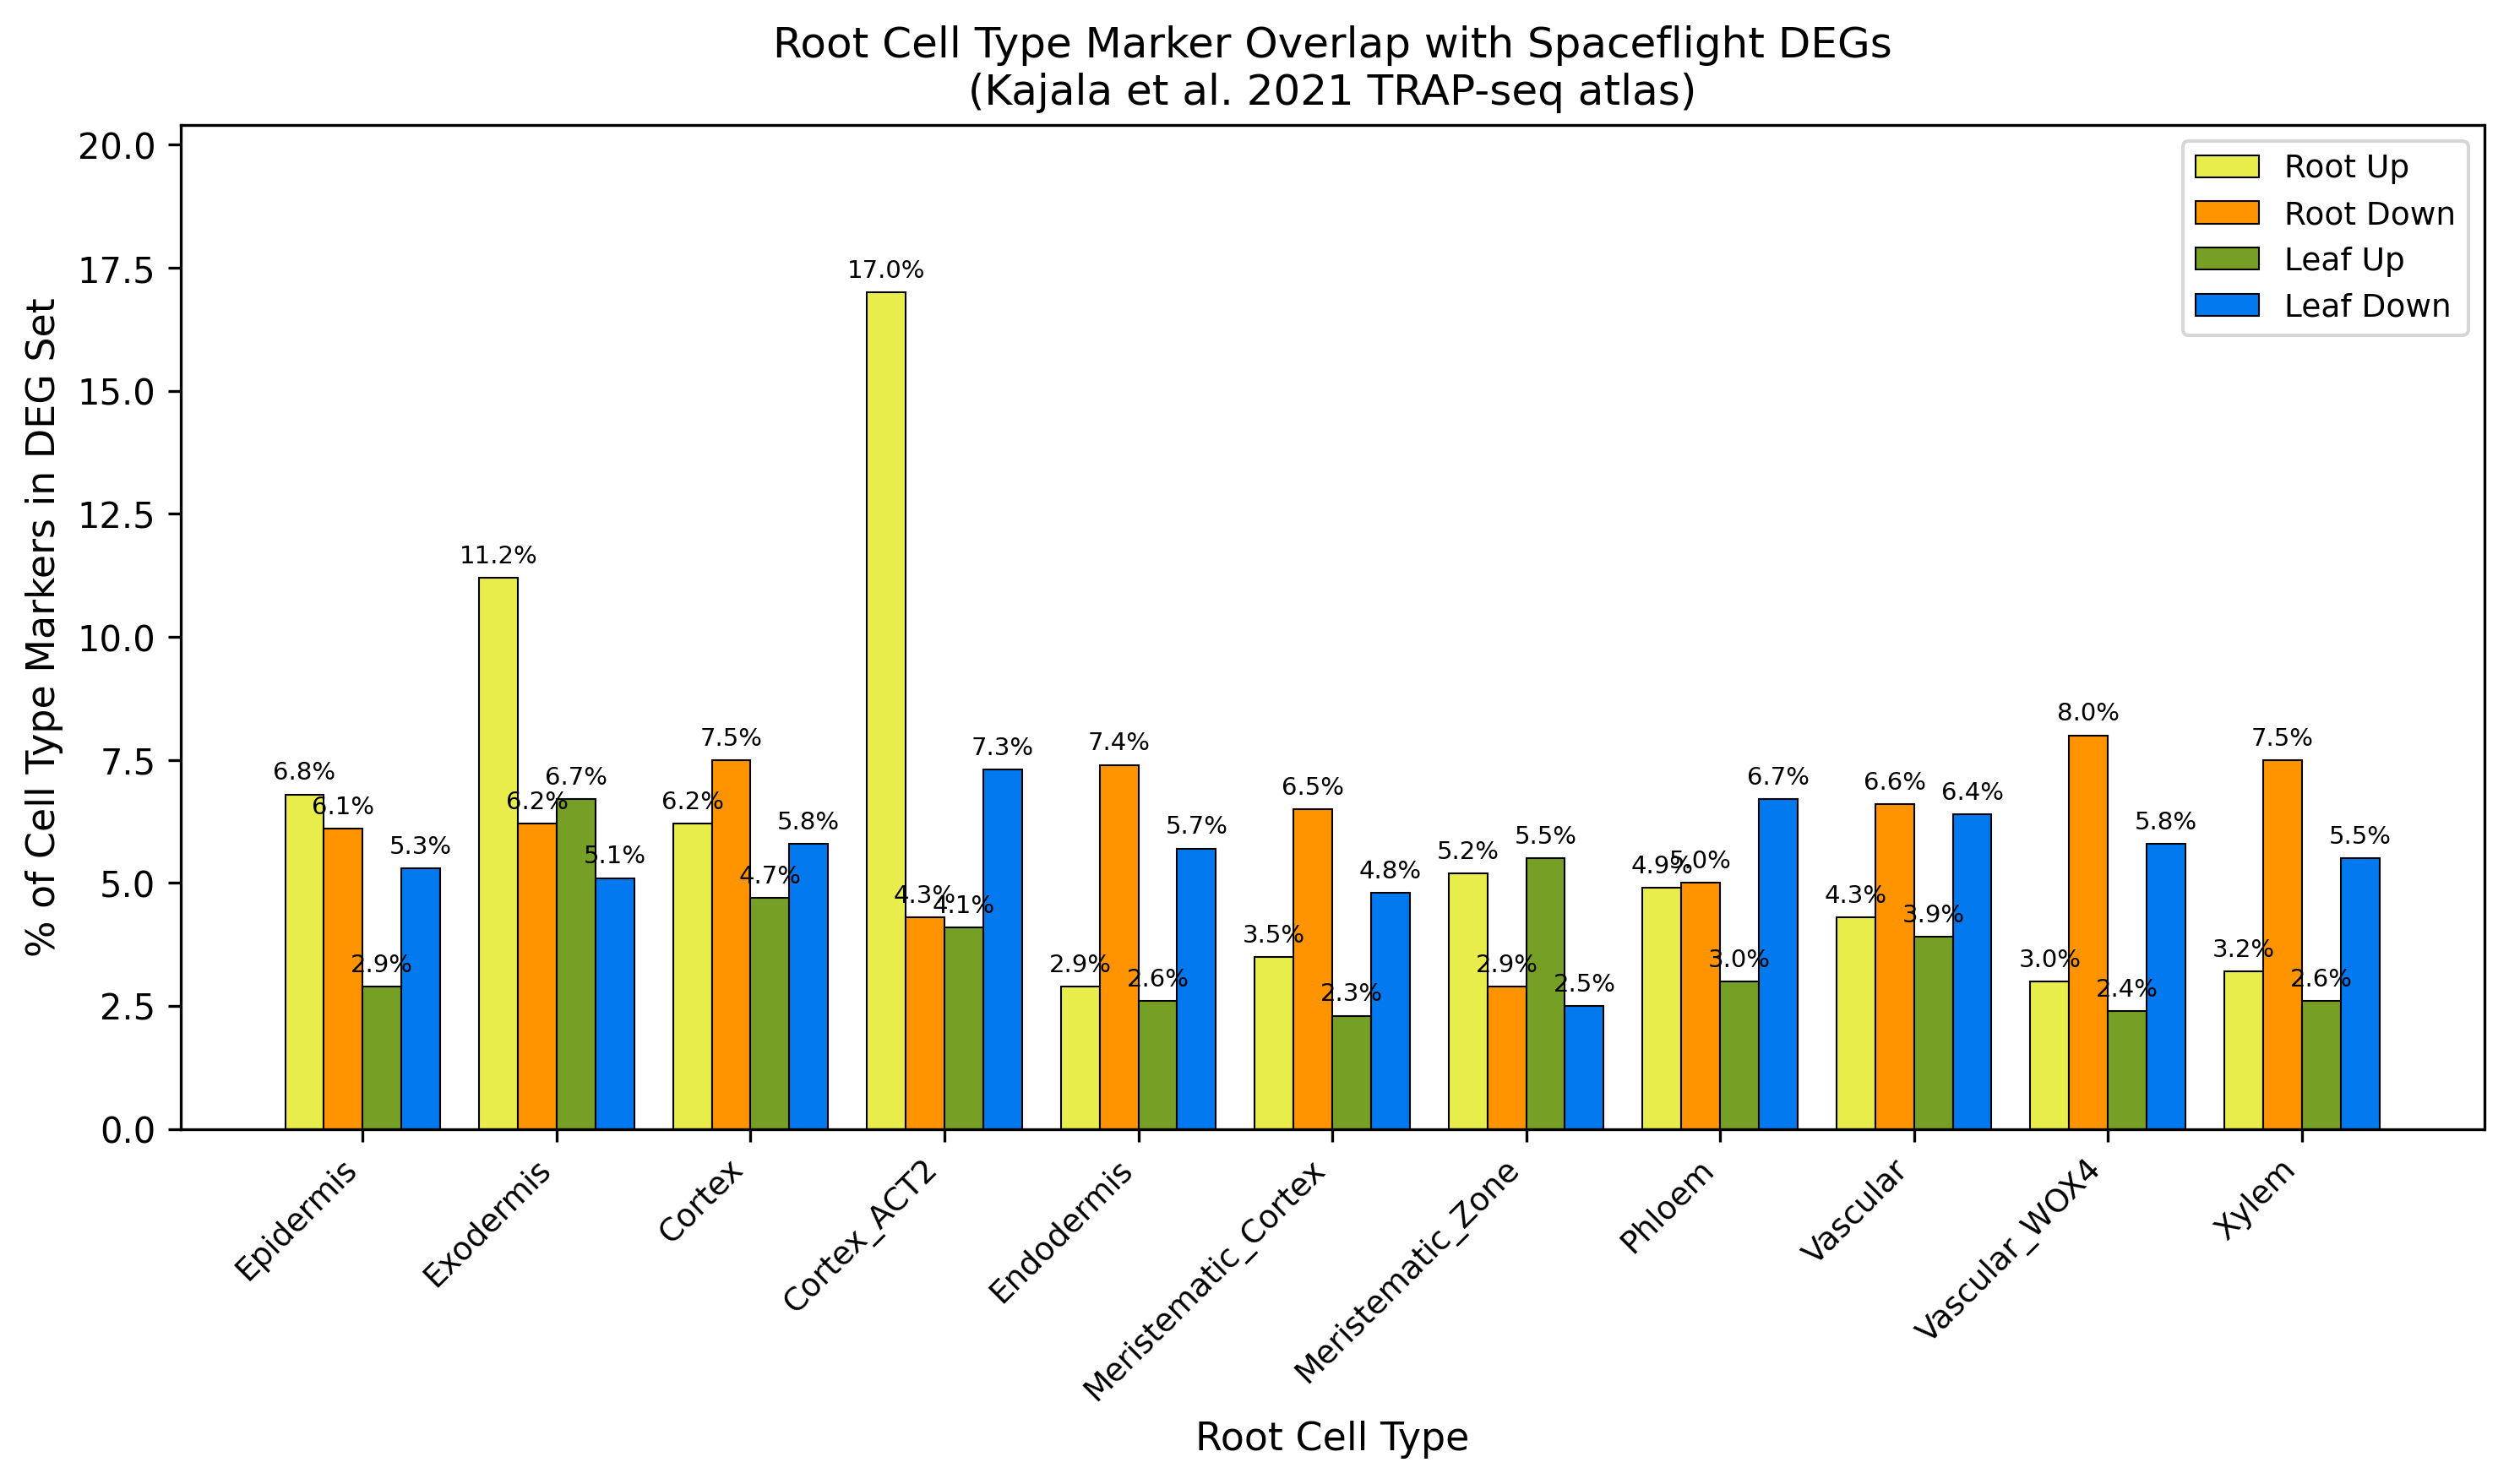
\includegraphics[width=\linewidth]{fig6c_root_celltype_bar.png}\caption{}\end{subfigure}
\caption{\textbf{Spaceflight root DEGs localise to ground-tissue and vascular cell
types.} Root DEGs cross-referenced against published tomato root cell-type
markers\cite{kajala2021} (Fisher's exact test, Bonferroni-corrected).
(\textbf{a})~Heatmap of $-\log_{10}$ adjusted $p$ for each cell type
(rows) $\times$ DEG set (columns); cortex is most enriched among down-regulated genes
(FDR $\approx 7\times10^{-29}$) and exodermis/Cortex\_ACT2 among up-regulated genes.
(\textbf{b})~Dot plot and (\textbf{c})~overlap bar plot summarising the same
associations.}
\label{fig:celltype}
\end{figure*}

% =====================================================================
\begin{table}[b]
\centering\small
\caption{\textbf{Differential expression summary (Flight vs Ground).} DESeq2 additive
model \texttt{$\sim$ light + condition}; DEGs at FDR $<0.05$, $|\log_2\text{FC}|\ge 1$.}
\label{tab:deg}
\begin{tabular}{lcccc}
\toprule
Tissue & $n$ & DEGs & Up & Down \\
\midrule
Leaf              & 21 & 2,132 & 1,032 & 1,100 \\
Adventitious root & 15 & 2,582 & 1,706 & \phantom{0}876 \\
\bottomrule
\end{tabular}
\end{table}

\end{document}
